%%%%%%%%%%%%%%%%%%%%%%%%%%%%%%%%%%%%%%%%%
% Masters/Doctoral Thesis 
% LaTeX Template
% Version 2.1 (2/9/15)
%
% This template has been downloaded from:
% http://www.LaTeXTemplates.com
%
% Version 2.0 major modifications by:
% Vel (vel@latextemplates.com)
%
% Original authors:
% Steven Gunn  (http://users.ecs.soton.ac.uk/srg/softwaretools/document/templates/)
% Sunil Patel (http://www.sunilpatel.co.uk/thesis-template/)
%
% License:
% CC BY-NC-SA 3.0 (http://creativecommons.org/licenses/by-nc-sa/3.0/)
%
%%%%%%%%%%%%%%%%%%%%%%%%%%%%%%%%%%%%%%%%%

%----------------------------------------------------------------------------------------
%	PACKAGES AND OTHER DOCUMENT CONFIGURATIONS
%----------------------------------------------------------------------------------------

\documentclass[
11pt, % The default document font size, options: 10pt, 11pt, 12pt
%oneside, % Two side (alternating margins) for binding by default, uncomment to switch to one side
english, % ngerman for German
singlespacing, % Single line spacing, alternatives: onehalfspacing or doublespacing
%draft, % Uncomment to enable draft mode (no pictures, no links, overfull hboxes indicated)
%nolistspacing, % If the document is onehalfspacing or doublespacing, uncomment this to set spacing in lists to single
%liststotoc, % Uncomment to add the list of figures/tables/etc to the table of contents
%toctotoc, % Uncomment to add the main table of contents to the table of contents
%parskip, % Uncomment to add space between paragraphs
]{MastersDoctoralThesis} % The class file specifying the document structure

\usepackage[utf8]{inputenc} % Required for inputting international characters
\usepackage[T1]{fontenc} % Output font encoding for international characters

\usepackage{palatino} % Use the Palatino font by default

\usepackage[backend=bibtex,natbib=false]{biblatex} % User the bibtex backend with the authoryear citation style (which resembles APA)

\addbibresource{example.bib} % The filename of the bibliography

\usepackage[autostyle=true]{csquotes} % Required to generate language-dependent quotes in the bibliography

%TODO aghosn
\usepackage[noend]{algpseudocode}
\usepackage{listings}
\usepackage{parcolumns}
\usepackage{xcolor}

\newcommand{\includecode}[2][c]{\lstinputlisting[caption=#2,escapechar=, style=custom#1]{#2}}

\lstdefinestyle{customc}{
  belowcaptionskip=1\baselineskip,
  breaklines=true,
  frame=single,
  xleftmargin=\parindent,
  language=C,
  showstringspaces=false,
  basicstyle=\footnotesize\ttfamily,
  keywordstyle=\bfseries\color{green!40!black},
  commentstyle=\itshape\color{purple!40!black},
  identifierstyle=\color{blue},
  stringstyle=\color{orange},
  tabsize=2,
  captionpos=b,
}

\lstdefinestyle{customasm}{
  belowcaptionskip=1\baselineskip,
  frame=L,
  xleftmargin=\parindent,
  language=[x86masm]Assembler,
  basicstyle=\footnotesize\ttfamily,
  commentstyle=\itshape\color{purple!40!black},
  captionpos=b,
}

\lstset{escapechar=@,style=customc}
%----------------------------------------------------------------------------------------
%	THESIS INFORMATION
%----------------------------------------------------------------------------------------

\thesistitle{Efficient Deoptimization} % Your thesis title, this is used in the title and abstract, print it elsewhere with \ttitle
\supervisor{Prof. Jan \textsc{Vitek}, Prof. Viktor \textsc{Kuncak}} % Your supervisor's name, this is used in the title page, print it elsewhere with \supname
\examiner{} % Your examiner's name, this is not currently used anywhere in the template, print it elsewhere with \examname
\degree{Master in Computer Science} % Your degree name, this is used in the title page and abstract, print it elsewhere with \degreename
\author{Adrien \textsc{Ghosn}} % Your name, this is used in the title page and abstract, print it elsewhere with \authorname
\addresses{6a rue de la Saint Martin, Saint Julien en Genevois, 74160, FRANCE} % Your address, this is not currently used anywhere in the template, print it elsewhere with \addressname

\subject{Computer Science} % Your subject area, this is not currently used anywhere in the template, print it elsewhere with \subjectname
\keywords{} % Keywords for your thesis, this is not currently used anywhere in the template, print it elsewhere with \keywordnames
\university{\href{https://www.epfl.ch/}{Ecole Polytechnique Federale de Lausanne}} % Your university's name and URL, this is used in the title page and abstract, print it elsewhere with \univname
\department{\href{http://ic.epfl.ch/computer-science}{Computer Science}} % Your department's name and URL, this is used in the title page and abstract, print it elsewhere with \deptname
\group{\href{http://lara.epfl.ch/w/}{LARA}} % Your research group's name and URL, this is used in the title page, print it elsewhere with \groupname
\faculty{\href{http://faculty.university.com}{Faculty Name}} % Your faculty's name and URL, this is used in the title page and abstract, print it elsewhere with \facname

\hypersetup{pdftitle=\ttitle} % Set the PDF's title to your title
\hypersetup{pdfauthor=\authorname} % Set the PDF's author to your name
\hypersetup{pdfkeywords=\keywordnames} % Set the PDF's keywords to your keywords

\begin{document}

\frontmatter % Use roman page numbering style (i, ii, iii, iv...) for the pre-content pages

\pagestyle{plain} % Default to the plain heading style until the thesis style is called for the body content

%----------------------------------------------------------------------------------------
%	TITLE PAGE
%----------------------------------------------------------------------------------------

\begin{titlepage}
\begin{center}

\textsc{\LARGE \univname}\\[1.5cm] % University name
\textsc{\Large Master Thesis}\\[0.5cm] % Thesis type

\HRule \\[0.4cm] % Horizontal line
{\huge \bfseries \ttitle}\\[0.4cm] % Thesis title
\HRule \\[1.5cm] % Horizontal line
 
\begin{minipage}{0.4\textwidth}
\begin{flushleft} \large
\emph{Author:}\\
\href{http://www.johnsmith.com}{\authorname} % Author name - remove the \href bracket to remove the link
\end{flushleft}
\end{minipage}
\begin{minipage}{0.4\textwidth}
\begin{flushright} \large
\emph{Supervisor:} \\
\href{http://www.jamessmith.com}{\supname} % Supervisor name - remove the \href bracket to remove the link  
\end{flushright}
\end{minipage}\\[3cm]
 
\large \textit{A thesis submitted in fulfilment of the requirements\\ for the degree of \degreename}\\[0.3cm] % University requirement text
\textit{in the}\\[0.4cm]
\groupname\\\deptname\\[2cm] % Research group name and department name
 
{\large \today}\\[4cm] % Date
%\includegraphics{Logo} % University/department logo - uncomment to place it
 
\vfill
\end{center}
\end{titlepage}

%----------------------------------------------------------------------------------------
%	DECLARATION PAGE
%----------------------------------------------------------------------------------------

\begin{declaration}
\addchaptertocentry{\authorshipname}

\noindent I, \authorname, declare that this thesis titled, \enquote{\ttitle} and the work presented in it are my own. I confirm that:

\begin{itemize} 
\item This work was done wholly or mainly while in candidature for a research degree at this University.
\item Where any part of this thesis has previously been submitted for a degree or any other qualification at this University or any other institution, this has been clearly stated.
\item Where I have consulted the published work of others, this is always clearly attributed.
\item Where I have quoted from the work of others, the source is always given. With the exception of such quotations, this thesis is entirely my own work.
\item I have acknowledged all main sources of help.
\item Where the thesis is based on work done by myself jointly with others, I have made clear exactly what was done by others and what I have contributed myself.\\
\end{itemize}
 
\noindent Signed:\\
\rule[0.5em]{25em}{0.5pt} % This prints a line for the signature
 
\noindent Date:\\
\rule[0.5em]{25em}{0.5pt} % This prints a line to write the date
\end{declaration}

\cleardoublepage

%----------------------------------------------------------------------------------------
%	QUOTATION PAGE
%----------------------------------------------------------------------------------------

\vspace*{0.2\textheight}

\noindent\enquote{\itshape Thanks to my solid academic training, today I can write hundreds of words on virtually any topic without possessing a shred of information, which is how I got a good job in journalism.}\bigbreak

\hfill Dave Barry

%----------------------------------------------------------------------------------------
%	ABSTRACT PAGE
%----------------------------------------------------------------------------------------

\begin{abstract}
\addchaptertocentry{\abstractname} % Add the abstract to the table of contents

The Thesis Abstract is written here (and usually kept to just this page). The page is kept centered vertically so can expand into the blank space above the title too\ldots

\end{abstract}

%----------------------------------------------------------------------------------------
%	ACKNOWLEDGEMENTS
%----------------------------------------------------------------------------------------

\begin{acknowledgements}
\addchaptertocentry{\acknowledgementname} % Add the acknowledgements to the table of contents

The acknowledgements and the people to thank go here, don't forget to include your project advisor\ldots

\end{acknowledgements}

%----------------------------------------------------------------------------------------
%	LIST OF CONTENTS/FIGURES/TABLES PAGES
%----------------------------------------------------------------------------------------

\tableofcontents % Prints the main table of contents

\listoffigures % Prints the list of figures

\listoftables % Prints the list of tables

%----------------------------------------------------------------------------------------
%	ABBREVIATIONS
%----------------------------------------------------------------------------------------

\begin{abbreviations}{ll} % Include a list of abbreviations (a table of two columns)


\end{abbreviations}

%----------------------------------------------------------------------------------------
%	SYMBOLS
%----------------------------------------------------------------------------------------

\begin{symbols}{lll} % Include a list of Symbols (a three column table)

%Symbol & Name & Unit \\

\addlinespace % Gap to separate the Roman symbols from the Greek

$\omega$ & angular frequency & \si{\radian} \\

\end{symbols}

%----------------------------------------------------------------------------------------
%	DEDICATION
%----------------------------------------------------------------------------------------

\dedicatory{For/Dedicated to/To my\ldots} 

%----------------------------------------------------------------------------------------
%	THESIS CONTENT - CHAPTERS
%----------------------------------------------------------------------------------------

\mainmatter % Begin numeric (1,2,3...) page numbering

\pagestyle{thesis} % Return the page headers back to the "thesis" style

% Include the chapters of the thesis as separate files from the Chapters folder
% Uncomment the lines as you write the chapters

% Chapter 1

\chapter{Introduction} % Main chapter title

\label{Chapter1} % For referencing the chapter elsewhere, use \ref{Chapter1} 

%----------------------------------------------------------------------------------------

% Define some commands to keep the formatting separated from the content 
\newcommand{\keyword}[1]{\textbf{#1}}
\newcommand{\tabhead}[1]{\textbf{#1}}
\newcommand{\code}[1]{\texttt{#1}}
\newcommand{\file}[1]{\texttt{\bfseries#1}}
\newcommand{\option}[1]{\texttt{\itshape#1}}

%----------------------------------------------------------------------------------------

Dynamic languages, such as JavaScript, Ruby, Python or R, often suffer from poorer performances than statically typed languages, like C, Java or C\#.
This disparity has multiple causes, among which the execution at runtime of many common programming language constructs, e.g., type tests and method dispatch, that static languages are able to evaluate during compilation.
In order to improve dynamic languages performance, language designers have started to investigate ways to shift the compilation later in a program's execution, by relying on just-in-time compilers.
Since in dynamic languages, little is known about the program ahead of time, a just-in-time compiler relies on runtime profiling data to perform adaptative optimizations and generate efficient compiled code at runtime.
The set of optimizations enabled in a JIT compiler are often more restricted than in a static compiler, where the entire program is available during the compilation.
For example, in a static compiler, function $g$ in Figure \ref{fig:example} can be type-checked, $H$ and $f$ are known, and their calls can be inlined and optimized.
In a dynamic language, $H$ and $f$ might not be yet defined or can be modified, their types are unknown, and no optimization can be performed.
As a result, new techniques are needed to lift restrictions in JIT compilers, and enable more agressive, speculative optimizations.\\

\begin{figure}[h]
\includecode{Code/Example.cpp}
\caption{Example.}
\label{fig:example}
\end{figure}
REFORMULATE ASSUME SOMETHING\\

On-stack replacement (OSR) is a concept that consists in replacing a program that is executing, by another program, while preserving the execution state.
Being able to switch between different programs, at runtime, while preserving the progress made so far by the execution, enables to implement aggressive speculative optimizations in JIT compilers.
The lack of information about the program's content is compensated by allowing the compiler to take any assumption about the program, and perform optimizations based on this assumption.
Whenever the assumption fails at runtime, the invalidated compiled program is replaced by a correct version, which resumes the execution.\\

\begin{wrapfigure}[13]{l}{6.5cm}
\includecode{Code/Example2.cpp}
\caption{Optimized versions.}
\end{wrapfigure}
Using OSR, a JIT compiler can assume that $H$ will not be redefined, and inline it during the JIT compilation of $g$.
It can further resolve $p$ and $y$, type-check them, and optimize the computation of $t * (3 ^ 4)$.
Whenever the assumption fails, e.g., $f$ triggers a redefinition of $H$, OSR allows to stop the execution of the program between lines 9 and 10, extract the state, and replace the function with the unsugared version.
The execution resumes at line 9 in Figure \ref{fig:example}.
On-stack replacement implementations are state-of-the-art features in advanced virtual machines and JIT compilers.\\


The R programming language suffers from very poor performances\cite{morandat2012evaluating}. 
It further exhibits a lazy evaluation of dynamically typed elements which prevents many common compiler optimizations from being performed.
Even worse, performance bottlenecks in R are intimately linked to R semantics. 
A JIT compiler for R, equipped with an efficient OSR implementation, could lift such restrictions, by generating more efficient unsound code, while preserving the correctness of the program.
The focus of this thesis is to provide an OSR implementation in RJIT, a JIT compiler for R, that enables to perform speculative optimizations while preserving the correctness of the program's execution.
The next section gives an overview of our solution and its implementation.\\

\section{Proposed Solution}
%First is overview of OSR implementations
%Second OSR deoptimization for RJIT compiler
%Third a speculative inliner to test the design
The first contribution of this thesis is an overview and synthesis of existing on-stack replacement implementations.
This thesis describes in details the main approaches taken to implement OSR, and their advantages and drawbacks.\\

The second and main contribution of this thesis is the implementation of RJIT OSR, an efficient OSR mechanism in the RJIT compiler for R, that enables agressive speculative optimizations while preserving the correctness of the program.
The implementation focuses on the on-stack replacement deoptimization mechanism in RJIT, and strives to provide code instrumentation with as little overhead as possible.
RJIT OSR prototypes a mechanism that could, in the future, enable to remove performance bottlenecks that are specific to R semantics.\\

The third and final contribution of this thesis is the implementation of an OSR-based speculative inliner in RJIT.
Function call inlining presents an interesting challenge in R, that requires to consider most of R and RJIT specificities.
The OSR inliner is used to evaluate our OSR implementation and provides an example of an interesting use of the OSR concept in an R compiler.\\

\section{Paper Overview}

The rest of this thesis is organized as follows: Chapter \ref{Chapter2} provides an overview of the on-stack replacement concept, defines OSR related vocabulary, and gives a high-level description of OSR mechanisms.
Chapter \ref{Chapter3} presents related work, i.e., implementations of OSR mechanisms in different virtual machines. It also provides a classification summary that regroups the differences between each implementation.
Chapter \ref{Chapter4New} describes RJIT OSR, the implementation of efficient OSR deoptimization in the RJIT compiler for R.
Chapter \ref{Chapter5} presents experimental results obtained with a speculative inliner, based on RJIT OSR.
Finally, Chapter \ref{Chapter6} concludes and presents ideas for future work.\\ 






% Chapter 2

\chapter{Related Work} % Main chapter title

\label{Chapter2} % For referencing the chapter elsewhere, use \ref{Chapter2} 

%----------------------------------------------------------------------------------------

% Define some commands to keep the formatting separated from the content 
\newcommand{\keyword}[1]{\textbf{#1}}
\newcommand{\tabhead}[1]{\textbf{#1}}
\newcommand{\code}[1]{\texttt{#1}}
\newcommand{\file}[1]{\texttt{\bfseries#1}}
\newcommand{\option}[1]{\texttt{\itshape#1}}

%----------------------------------------------------------------------------------------

\section{On Stack Replacement, General Principle}

\subsection{Definition \& Overview}
%Replace some portion of code while it is executing 
%Used to optimise code that is running 
%Used to undo an invalid optimisation of the code that is running
On-Stack replacement (OSR) is a set of techniques that consist in dynamically transferring the execution, at run time, between different pieces of code.
The action of transferring the execution to another code artefact is called an OSR transition.\\

On-Stack replacement can be viewed, at a high level, as a mechanism that allows to transform the currently executing code, into another version of itself.
This transformation mechanism has been used to allow the bi-directional transition between different levels of code optimisations.
We can therefore reduce it to two main purposes: transforming an executing piece of code into a more optimised version of itself, and undoing transformations that were previously performed.
While similar, these two types of transformation have very different goals.\\

In several virtual machines (CITE PAPERS), some of which will be presented in (REFERENCE), On-Stack replacement has been used to improve the performance of long running functions.
When the VM identifies a piece of code as being "hot", i.e., it hogs the execution, it suspends its execution, recompiles it to a higher level of optimisation, and transfers the execution to the newly generated version of the function.
This differs from a simple Just-In-Time (JIT) compiler, since the recompilation takes place during the execution of the function, rather than just before its execution.
%TODO reformulate
However, both techniques rely on run time profiling data to uncover new optimisation opportunities.
In this case, OSR is used to improve performance.\\

On-Stack replacement allows a compiler to perform speculative transformations.
Some optimisations rely on assumptions that are not bound to hold during the entire execution of a program.
A simple example is function inlining in an environment where functions can be redefined at any time.
A regular and correct compiler would not allow to inline a function that might be modified during the execution.
The OSR mechanism, on the other hand, enables to perform such an optimisation.
Whenever the assumption fails, i.e., the function is redefined, the OSR mechanism will enable to transfer the execution to a corresponding piece of code where the inlining has not been performed.
In this case, OSR is used to preserve correctness.\\

On-Stack replacement is a powerful technique, that can be used to either improve performance, or enable speculative transformations of the code while preserving correctness.
In the next subsection, we present the historical origins of On-Stack replacement and detail its most interesting features.\\ %TODO don't like the word feature
  

\subsection{The origins: SELF debugging}
%SELF needs aggressive optimisations to have reasonable performance. 
%But that prevents from debugging
%Hence OSR enables selective deoptimization at runtime, which provides source level information 
%That makes some optimisations not available since they are hard to undo (e.g. tail %recursion elimination)
%Scope descriptors enable mapping between optimised and unoptimised, enables to keep track %of the position in the virtual call tree etc. (will be detailed). 
%Interrupt points (where, why, how)
%Function invalidation
The SELF programming language is a pure object-oriented programming language.
SELF relies on a pure message-based model of computation that, while enabling high expressiveness and rapid prototyping, impedes the languages performances(CITE from self paper).
Therefore, the language's implementation depends on a set of aggressive optimisations to achieve good performances(CITE).
SELF provides an interactive environment, based on interpreter semantics at compiled-code speed performances.\\
Providing source level code interactive debugging is hard in the presence of optimisations.
Single stepping or obtaining values for certain source level variables might not be possible.
For a language such as SELF, that heavily relies on aggressive optimisations, implementing a source code level debugger requires new techniques.\\
In (CITE Holzle), the authors came up with a new mechanism that enables to dynamically de-optimise code at specific interrupt points in order to provide source code level debugging while preserving expected behaviour (CITE from holzle).\\

\subsection{Why is OSR interesting?}
%The optimisation case
     %wait until enough profiling information is gathered to make some new assumptions and improve code quality
    %Some enable to have several specialised versions of the code live at the same time.
    %Chaining OSR means that we can keep optimising the code
%The deoptimization case
    %This is the real deal. Optimisation is not valid without this counter part. 
    %Enables even more agressive code specialisation. Being able to undo means that we can have virtually any assumption and just revert back to a safe version if it fails. 
    %The real difference: optimisation is for performance, deoptimazation is for correctness.


\section{On Stack Replacement \& Virtual Machines}
\subsection{In Java}
%Java Hotspot 
%Graal 
%Jikes

\subsection{LLVM}
%What is LLVM? 
    %Some description of LLVM, putting the emphasis on the fact that it enables to generate native code from LLVM IR, and that many languages have an LLVM compiler (e.g. R, Ruby, Python, Matlab etc.) 
    %Provides tools and mechanism that we can reuse (e.g. low level optimisations, passes on the code etc.) 
%Why OSR on LLVM? 
    %General technique that can be profitable to several languages. 
    %Don’t need to worry about static optimisations 
    %Get portability for free
    %Examples: Webkit & McJit

%probably move that somewhere else
\section{A Description of Existing Implementations}
\subsection{The OSR points}
%Several names for it 
%what it is: a point in the code from which we can suspend the exec and optimise the current version of the code
    %Implies that we need a "safe state”, i.e., we need to be able to find an equivalent point in the optimised version
    %portions of code that don’t have interrupts
%Guarded vs Unguarded 
    %Guarding when there is an explicit condition that we can check locally
    %What if global/External event? 
        %Some have a map of such points and fix them whenever an external event happens (citing papers e.g., jikes)
%OSR exits 
    %What to do when the condition fails? 
        %Optimisation dependent 
        %for external requires to correct every callee return landing spots. 
        %Requires corresponding entry in the unoptimised version
%Examples from existing implementations 
    %MCJIt inserter and instrument passes (need a code transformer + OSR Label)
    %Jikes
\subsection{The Transition Mechanism}
%The ideal model 
    %Being able to stop execution, save the state, generate a new version, fix the state, replace the instruction pointer and resume.
%The more reasonable case of function calls 
    %Implemented as a function call 
    %In SELF: data structures on the side to keep mapping between virtual and physical (might be redundant with 2.1.2)
    %Jikes: the VARMAP that enables to do it virtually at and across OSR points, registers state etc. 
    %MCJit: Saving all live variables, instruments code to jump to correct spot in new version by instrumenting the prolog of the function + executing a special block to fix the state etc. 
    %Rome & Others (to be defined): pass everything as arguments, do a function call and instrument entry point of the function to fix the state and jump to correct continuation point.  

\subsection{Constraints and Limitations}
%Limits the types of optimisations that can be performed (e.g. tail recursion elimination in SELF) 
%Limits code motion + Mechanisms extend variable live range
%Limited spots where we can perform the transition, often limited to function pro/epilogues and loops  
    %Due to the difficulty of finding/ensuring a mapping between optimised and unoptimised otherwise. 
%The space complexity 
    %need to keep additional information around (e.g. variables that were eliminated need to be correctly re-generated when deoptimizing)
    %Instrumentation increases the code
\subsection{Generating on the Fly VS Caching}
%Caching enables to keep several versions around + saves compilation time
%On the fly: we can keep the same address for the function

\subsection{Discussion}
%The proposed classification in MCJit (several optimisation, possible deoptimization) 
%The trade off between performance gain and the compilation & instrumentation costs. 
%The paradoxal goal of finding a general technique to aggressively specialise code in particular assumption based circumstances. 
    %By being too general, we actual bring limitations to the implementation 
    %Assumption based optimisations need to be implemented for the OSR mechanism (e.g., mcjit “transformer” method) 
        %How to find a correct API that satisfies every possible optimisation that we might want to perform? 
            %Support external event
            %Support guards
%The challenge of code motion 




% Chapter 3

\chapter{Related Work} % Main chapter title

\label{Chapter3} % For referencing the chapter elsewhere, use \ref{Chapter2} 

%----------------------------------------------------------------------------------------

% Define some commands to keep the formatting separated from the content 
\newcommand{\keyword}[1]{\textbf{#1}}
\newcommand{\tabhead}[1]{\textbf{#1}}
\newcommand{\code}[1]{\texttt{#1}}
\newcommand{\file}[1]{\texttt{\bfseries#1}}
\newcommand{\option}[1]{\texttt{\itshape#1}}

%----------------------------------------------------------------------------------------
\section{The origins: SELF Debugging}\label{SELF}
%SELF needs aggressive optimizations to have reasonable performance. 
%But that prevents from debugging
%Hence OSR enables selective deoptimization at runtime, which provides source level information 
%That makes some optimizations not available since they are hard to undo (e.g. tail %recursion elimination)
%Scope descriptors enable mapping between optimized and unoptimized, enables to keep track %of the position in the virtual call tree etc. (will be detailed). 
%Interrupt points (where, why, how)
%Function invalidation
SELF is a pure object-oriented programming language.
It relies on a pure message-based model of computation that, while enabling high expressiveness and rapid prototyping, impedes the languages performances(CITE from self paper).
As a result, the language's implementation depends on a set of aggressive optimizations to achieve good performances\cite{holzle1992debugging}.
SELF provides an interactive environment, based on interpreter semantics at compiled-code speed performances.\\

Providing source level code interactive debugging is hard in the presence of optimizations.
Single stepping or obtaining values for certain source level variables might not be possible.
For a language such as SELF, that heavily relies on aggressive optimizations, implementing a source code level debugger requires new techniques.\\

In \citetitle{holzle1992debugging}\cite{holzle1992debugging}, the authors came up with a new mechanism that enables to dynamically de-optimize code at specific interrupt points in order to provide source code level debugging while preserving expected behaviour (CITE from holzle).\\

\citean{holzle1992debugging} present the main challenges encountered to provide debugging behaviours, due to the optimizations performed by the SELF compiler. 
Displaying the stack according to a source-level view is impeded by optimizations such as inlining, register allocation and copy propagation.
For example, when a function is inlined at a call site, only a single activation frame is visible, while the source level code expects to see two of them.
Figure (FIG), taken from \cite{holzle1992debugging}, provides another example of activations discordances between physical and source-level stacks.
In this figure, the source-level stack contains activations that were inlined by the compiler. For example, the activation B is inlined into A', hence disappearing from the physical stack.\\
\begin{figure}[h]
\centering
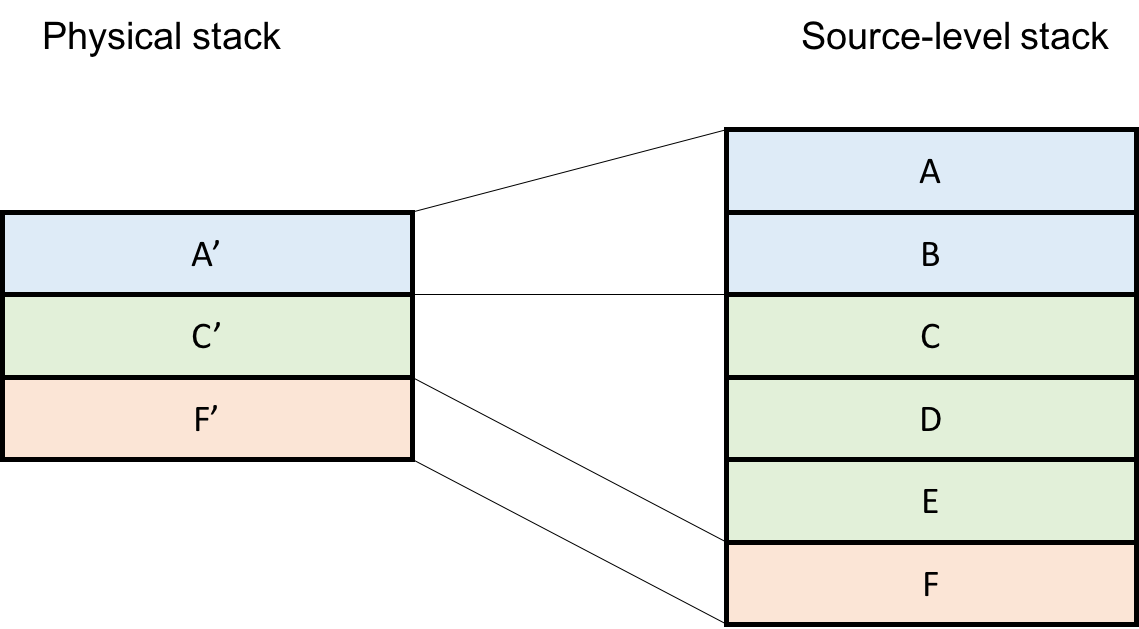
\includegraphics[scale=0.5]{Figures/Figure1}
\decoRule
\caption[physical vs. source-level stacks]{Displaying the stack, figure from \cite{holzle1992debugging}.}
\end{figure}

Single-stepping is another important feature for a debugger. 
It requires to identify and execute the next machine instruction that corresponds to the source operation.
\citean{holzle1992debugging} highlight the impact of code motion and instruction scheduling on the machine instruction layout. 
Such optimizations re-order, merge, intersperse and sometimes delete source-level operations, therefore preventing a straight forward implementation of single-stepping for the debugger.\\

Compiler optimizations prevent dynamic changes from being performed in the debugger.
Holzle(CITE) identifies two separate issues: changing variable values, and modifying procedures (i.e., functions).
To illustrate the first case, Holzle CITE relies on an example where a variable is assigned the sum of two other variables.
The compiler identifies the two variables as being constants and replaces the addition by a direct constant assignment.
A debugger that allows to change variable values at run time would then yield a non correct behaviour if the user modifies one of the two variables. 
This problem does not arise in the case of unoptimized code since the addition is still present. 
For procedures, Holzle CITE describes an example where a function has been inlined by the compiler, but redefined by the user in the debugger.\\

Holzle(CITE) distinguishes two possible states for compiled code: \textit{optimized}, which can be suspended at widely-spaced interrupt points, from which we can reconstruct source-level state, and \textit{unoptimized}, that can be suspended at any source-level operation and is not subjected to any of the above debugging restrictions.\\

In order to deoptimize code on demand, SELF debugger needs to recover the unoptimized state that corresponds to the current optimized one. 
To do so, it relies on a special data structure, called a \textit{scope descriptor}. 
The scope descriptors are generated during compilation for each source-level scope. 
This data structure holds the scope place in the virtual call tree of the physical stack frame and records locations and values of its argument and local variables. 
It further holds locations or values of its subexpressions.
Along with the scope descriptor, the compiler generates a mapping between virtual (i.e, scope descriptor and source position within the scope) and physical program counters (PC).
Figure \ref{Holzle2} is taken from CITE and displays a method suspended at two different points. 
At time t1, the stack trace from the debugger displays frame B, hiding the fact that B was inlined inside of A.
At time t2, D is called by C which is called by A, hence, the debugger displays 3 virtual stack frames instead of only one physical frame.\\

\begin{figure}[h]
\centering
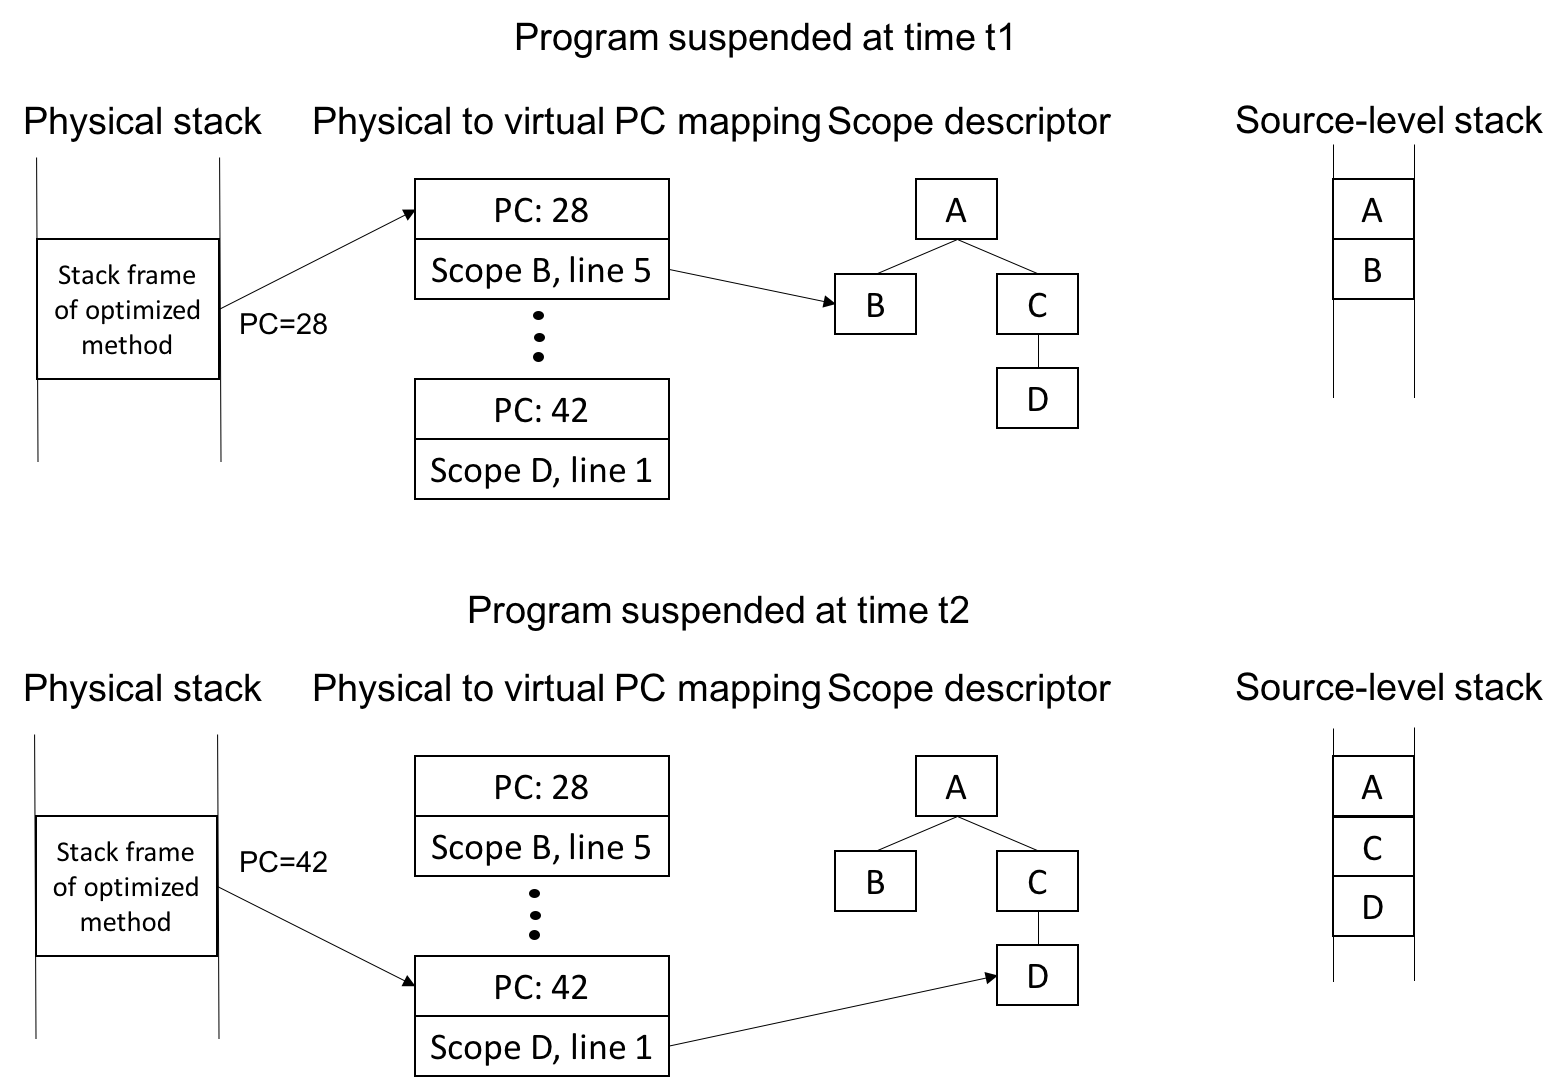
\includegraphics[scale=0.5]{Figures/Figure2}
\decoRule
\caption[Recovering the source-level state]{Recovering the source-level state (from CITE).}
\label{Holzle2}
\end{figure}


The de-optimization process follows 5 steps described in CITE and summed up here:
\begin{enumerate}
    \item Save the physical stack frame and remove it from the run time stack.
    \item Determine the virtual activations in the physical one, the local variables and the virtual PC.
    \item Generate completely unoptimized compiled methods an physical activations for each virtual one.
    \item Find the unique new physical PC for each virtual activation and initialise (e.g., return addresses and frame pointers) the physical activations created in the previous step.
    \item Propagate the values for all elements from the optimized to the unoptimized activations.
\end{enumerate}

Holzle(CITE) also describes \textit{lazy deoptimization}, a technique to deoptimize a stack frame that is not at the current top of the execution stack. 
Lazy deoptimization defers the deoptimization transformation until control is about to return into the frame, hence enabling deoptimization for any frame located on the stack.\\

Deoptimization at any instruction boundary is hard. 
It requires to be able to recover the state at every single point of the program.
Holzle (CITE) relies on a weaker easier restrictions by enabling deoptimization only at certain points called \textit{interrupt points}. 
At an interrupt point, the program state is guaranteed to be consistent. 
The paper (CITE) defines two kinds of interrupt points: method prologues, and backward branches (i.e., end of loop bodies).
Holzle(CITE) therefore estimates the length of the longest code sequence that cannot be interrupted to be a few dozen of instruction, i.e., the average length of a code sequence that does not contain neither a call nor a loop end.
Interrupt points are also inserted at all possible run time errors to allow better debugging of synchronous events such as arithmetic overflow. 
The generated debugging information are needed only at interrupt points, which reduces the space used to support basic debugger operations (as opposed to allowing interrupts at any instruction boundary).\\

Providing a debugger for SELF limits the set of optimizations that the compiler can support, and decreases the performances of the program when the execution is resumed. 
Tail recursion elimination saves stack space by replacing a function call with a goto instruction, while fixing the content of registers.
SELF debugger is unable to reconstruct the stack frames eliminated by this optimization and hence, it is not implemented in the SELF compiler.
More generally, tail call elimination is one important limitation for the SELF debugger.

The debugger slows down the execution when the user decides to resume. 
The execution should proceed at full speed, but some stack frames might have been unoptimized, hence implying that a few frames might run slowly right after resuming execution.\\

\section{OSR \& VMs}
Virtual machines are privileged environments in which On-Stack replacement can be used to its full power.
As seen in \ref{WhyOSRInteresting}, OSR is as useful as the compiler's profiler is efficient.
A virtual machine (VM) has control over the resources allocation, enables to control the code that is generated by the compiler, maintains important run time data, and state information about the program being executed.\\

This section presents several examples of VMs that support On-Stack replacement. 
The section is divided into two parts: we first presents several solutions that provide OSR for various virtual machines, then we briefly introduce LLVM, a VM presenting an interesting framework in which we believe On-Stack replacement mechanism should fit.\\ 

\subsection{HotSpot}\label{HotSpot}

The Java HotSpot Performance Engine(CITE web) is a Java virtual machine developed and maintained by Oracle.
The Java HotSpot VM provides features such as a class loader, a bytecode interpreter, Client and Server virtual machines, several garbage collectors, just-in-time compilation and adaptive optimizations.\\

The Java HotSpot Engine supports on-stack replacement in order to provide efficient deoptimization\cite{paleczny2001java}.
When a class loading invalidates an optimization decision, such as a call inlining, the methods relying on this decision need to be deoptimized.
Threads that are executing in a method that needs to be deoptimized are stopped as soon as they reach a safepoint.
The JVM state is recorded as an input of safepoints and procedure calls.
This implies, as a side effect, that the entire JVM state is marked as "live" at a safepoint, hence extending the live range of some values.
The Java HotSpot Engine then extracts the native frame corresponding to this execution trace, and converts it into a byte code interpreter frame.
The execution of the method then continues in the interpreter.
UNCOMMON TRAPS\\

\subsection{Jikes RVM}

The Jikes Research Virtual Machine (RVM)(REF) is an open source, self hosted, i.e., it is entirely implemented in Java, virtual machine for Java programs.
%TODO compile only from Qian.
It provides advanced state-of-the-art features such as dynamic compilation, adaptive optimizations, garbage collection, thread scheduling, and synchronization (CITE).\\

Jikes RVM is an extensible framework in which different On-Stack replacement techniques have been implemented.
%The first
\citean{fink2003design} implemented OSR support in JikesRVM. 
Their implementation relies on JVM scope descriptor, associated to method activation frames.
A scope descriptor contains the thread running the activation, the bytecode index that corresponds to the program counter, values of all local and stack locations, and a reference to the activation's stack frame.
The OSR transition is divided into three steps: 
\begin{enumerate}
    \item Extract the compiler-independent state from a suspended thread. 
    \item Generate the new code for the suspended activation.
    \item Transfer the execution in the suspended thread to a new compiled code.
\end{enumerate}
\citean{fink2003design} generates the target function by compiling a specialized version of the method for each activation that is replaced, as well as a new version for future invocations.
In other words, instead of allowing multiple entry points per function \cite{lameed2013modular, paleczny2001java}, this JikesRVM OSR implementation generates a specialized version of the target function that has only one entry point, corresponding to the instruction from which the OSR transition was triggered.
Each such method contains a special \textit{prologue}, responsible for saving values into locals and loading values on the stack.
OSR transitions can be taken at special points, called \textit{OSR points}, introduced by the optimizing compiler and that correspond to points where the running activation may be interrupted.
The implementation makes a distinction between unconditional and conditional OSR points.
An OSR point is implemented as a call that takes all live variables as arguments. 
This constraints some optimizations such as dead code elimination, load elimination, store elimination and code motion by extending the liveness scope of some variables.
An OSR point transfers control to an exit block, i.e., it can be viewed as a non-return call.\\

\citean{soman2006efficient} proposed a general-purpose OSR mechanism, for JikesRVM, that presents less restrictions for compiler optimizations than the previous approach, while decoupling the OSR implementation from the optimization process.
They extend the previous OSR implementation\cite{fink2003design} to enable OSR transition at, and accross points at which the execution can be suspended.
In order to do so, they rely on a special data structure called a \textit{variable map}(VARMAP).
A VARMAP is associated with each method, and consists in a list of thread-switching points and their live variables.
When the compiler performs optimizations, the VARMAP is updated accordingly.
Once the compilation completes, the VARMAP is encoded into a compressed map that contains an entry for each OSR point present in the method. EXPAND ON HOW OSR IS PERFORMED.
\citean{soman2006efficient} also propose an alternative lazy triggering of on-stack replacement.
Lazy triggering consists in taking an OSR transition due to events in the environment, i.e., events triggered by the runtime. 
Whenever the runtime deems an assumption invalide, it invokes a helper function called \textit{OSR helper} that either patches the code of the executing methods to call the OSR process, or it modifies return addresses of the callees of the method to be replaced to point to the OSR helper.
When a callee returns, the OSR helper creates a new stack frame with the state extracted from the specialized method's stack and saves all of the specialized method registers into its stack frame. 
The return address of the OSR helper points to the current instruction in the specialized code, which is then used during OSR to identify the location to resume the execution in the new version of the method.
Lazy triggering improves the code efficiency by avoiding the extra cost of guards evaluations.\\

EXPERIMENTAL RESULTS.

\subsection{WebKit VM}\label{webkit}

WebKit is an open source web browser engine used to improve JavaScript performances.
It exhibits a Four-Tier VM architecture. 
The WebKit run-time compilation flow is described by Figure \ref{FTL}.\\
\begin{figure}[h]
\centering
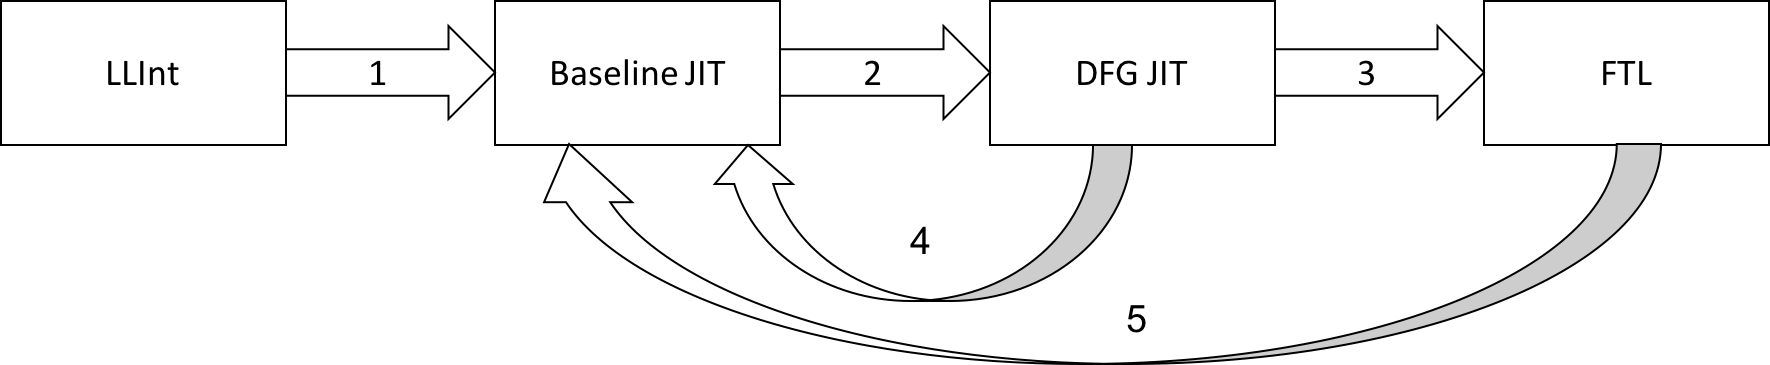
\includegraphics[scale=0.5]{Figures/FTL}
\decoRule
\caption[The WebKit FTL]{The WebKit Four-tier optimization flow.}
\label{FTL}
\end{figure}
 
Forward arrows represent \textit{OSR entries}, i.e., a transformation that yields a more optimized version of the code at run-time.
Backward arrows correspond to \textit{OSR exits}, i.e., a transformation that yields a less optimized version of the code at run-time.
The low level interpreter (LLInt) is used for low latency start up.
The baseline JIT generates WebKit bytecode with no optimization enabled.
The transition from the first tier to the second one happens when a statement is executed more than a hundred times or a function is called more than six times.
The data flow graph (DFG) JIT is triggered when a statement executes more than a thousand times or a function is called more than sixty-six times.
The FTL tier relies on LLVM machine code optimizations to generate a fast version of portions of the code.
In order to hide the costs of the translation to LLVM IR and its compilation time, the FTL is triggered only for long running portions of the code that are currently executing.
There are two kinds of transitions in WebKit: the ones contained entirely inside the WebKit framework (i.e., transitions 1,2 \& 4 in Figure \ref{FTL}), and the ones that involve LLVM (i.e., 3 \& 5 in Figure \ref{FTL}).\\

Transitions to and from LLVM are hard. 
There is no control over the stack layout or the optimized code produced by LLVM.
In the case of transition 3, a different LLVM version is generated for each entry point that the framework desires to have inside this function.
In WebKit, such entry points are located at loop headers. 
This choice makes sense with regard to the condition to enter the FTL, i.e., transition 3 is taken for long running portions of code that could be improved thanks to LLVM low level optimizations.
WebKit has to generate a different version for each entry points for two main reasons: LLVM allows only single entry points to functions (going around this limitation would require to modify LLVM IR and implementation), and instrumenting a function with several entry points would impact on the quality and performance of the generated native code by extending the code's length and restricting code motion.\\

Performing transition 3 requires to get the current state of execution and identify the entry point corresponding to the current instruction being executed.
The DFG dumps its state into a scratch buffer.
An LLVM function with the correct entry point is then generated, and instrumented such that its first block loads the content of the scratch buffer and correctly reconstructs the state.
The mapping between the DFG IR nodes and the LLVM IR values is straight forward since both IR's are in SSA.
A special data structure, called a Stackmap, enables to keep the mapping between LLVM values and registers/spill-slots.\\

Transition 5 is harder as it requires to extract the execution state from LLVM.
WebKit has two different mechanisms to enables OSR exits: the exit thunk and the invalidation points.
In the first case, WebKit introduces exit branches at OSR exit points.
The branch is guarded by an OSR exit condition and is a no-return tail call to a special function that takes all the live non-constant and not accounted for bytecode values.
The second mechanism enables to remove the guard.
Since we assume that the portion of code that is instrumented is executed a lot of times, the cost of testing the condition can have a great impact on the overall execution time.
This mechanism relies on special LLVM intrinsics, namely patchpoints and stackmap shadow bytes.
A patchpoint enables to reserve some extra space in the code, filled with nop sleds. 
When the WebKit framework detects that an exit should be taken, it overwrites the nop sleds with the correct function call to perform the OSR exit.
This breaks the optimized version of the code which cannot be re-used later on and must be collected.
The stackmap shadow bytes improves on this technique by allowing to directly overwrite the code, without having any nop sled generated before hand.

WebKit is a project that heavily, and successfully relies on OSR to improve performances.
The web browser engine is used in Apple Web browser Safari and enables a net improvement of performances why proving to be reliable(CITE?).
Although successful, it does not provide a general and reusable framework for OSR in LLVM that other projects could benefit from.\\

\section{OSR \& LLVM}\label{OSR&VM}
\subsection{What is LLVM?}
%TODO cite the llvm paper?
LLVM is a compiler infrastructure providing a set of reusable libraries.
LLVM provides the middle layers of a compiler system and a large set of optimizations for compile-time, link-time, run-time, and idle-time for arbitrary programming languages.
These optimizations are performed on an intermediate representation (IR) of the code and yield an optimized IR.
The LLVM framework also provides tools to convert and link code into machine dependent assembly code for a specific target platform.
LLVM supports several instruction sets including ARM, MIPS, AMD TeraScale, and x86/x86-64(CITE?).\\

The LLVM intermediary representation is a language-independent set of instructions that also provides a type system.
The LLVM IR is in static single assignment form (SSA), which requires every variable to be defined before it is used and assigned exactly once. 
SSA enables or improves several compiler optimizations among which constant propagation, value range propagation, sparse conditional constant propagation, dead code elimination, global value numbering, partial redundancy elimination, strength reduction and register allocation.
The SSA requirement for variables to be assigned only once requires a special mechanism, called a $\phi$-node, when a value depends on which control flow branch was executed before reaching the current variable definition.
Figure \ref{SSA example} provides an example where we have to choose between two possible values for a variable after the merging of two control flow branches.

\begin{figure}[h]
\centering
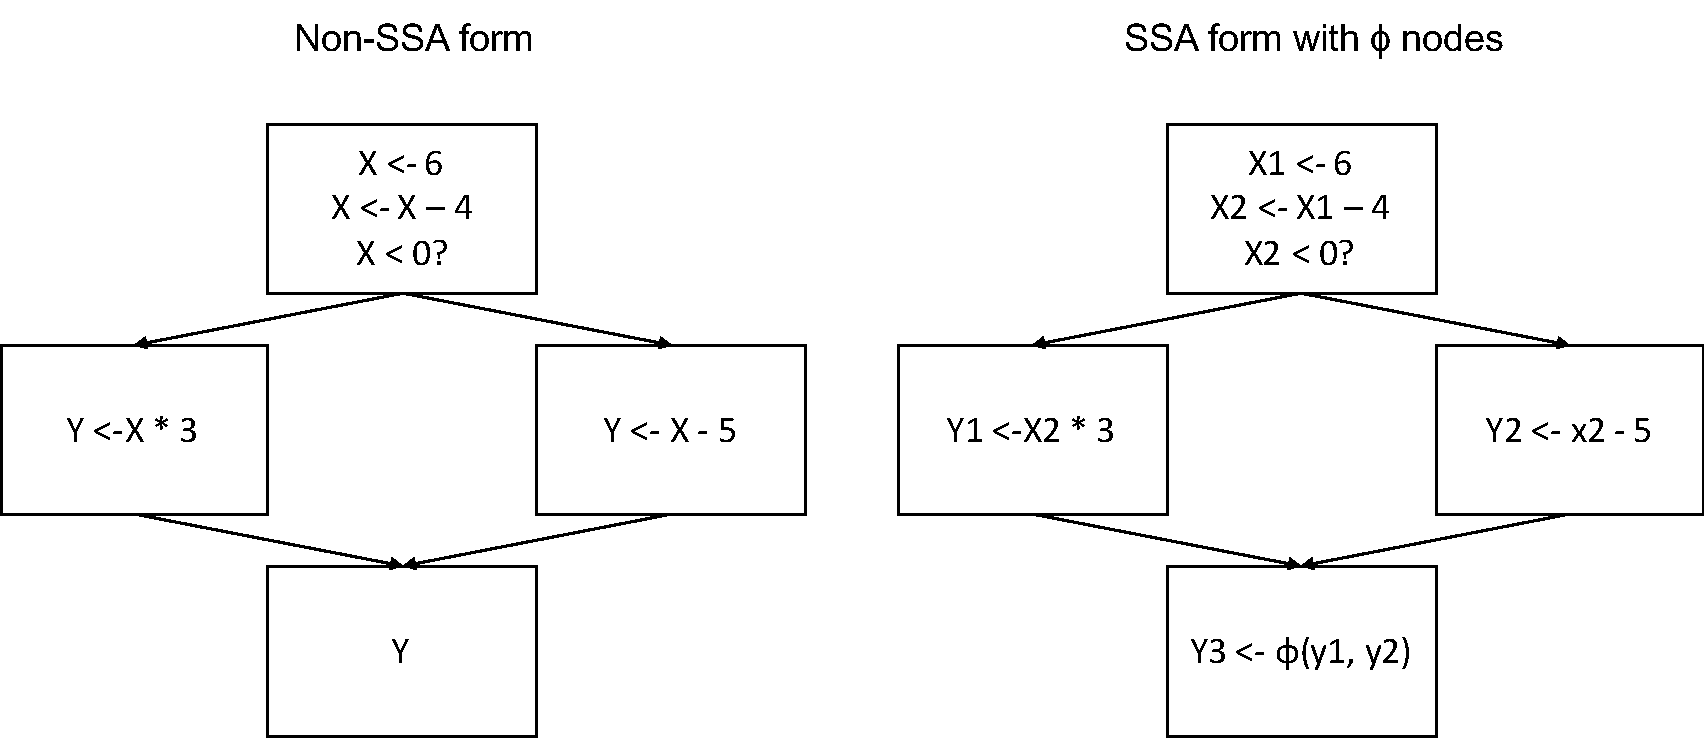
\includegraphics[scale=0.5]{Figures/SSAForm}
\decoRule
\caption[SSA example]{Example of $\phi$-node in SSA form.}
\label{SSA example}
\end{figure}

%TODO exhaustive basic types?
The LLVM IR type system provides basic types (e.g., integers, floats), and five derived types: pointers, arrays, vectors, structures, and functions.
Any type construct can then be represented as a combination of these types.\\

%TODO reformulate/restructure this §
The LLVM framework is a versatile tool that enables to implement many programming languages paradigms.
LLVM compilers exist for several mainstream/popular languages such as Java, Python, Objective-C, and Ruby have an LLVM compiler.
Other languages, like Haskell, Scala, Swift, Rust, Ada, and Fortran also have an LLVM compiler implementation.
LLVM basic types enable to support object-oriented languages, such as Java and Python, dynamically typed languages like R or statically typed like Scala.
LLVM also enables to model functional languages such as Haskell, as well as imperative ones. 
Furthermore, it supports reflection and, thanks to dynamic linking, modular languages (e.g., Haskell).
The tools provided enable static compilation as well as dynamic compilation techniques such as Just-In-Time compilation (JIT).\\

\subsection{Why do we want OSR in LLVM?}

On-Stack replacement high-level mechanism is language-independent.
Therefore, implementing OSR as a clean modular addition to LLVM would enable developers to leverage this feature in many programming languages, without requiring them to write a new compiler from scratch.
Furthermore, as explained in \ref{WhyOSRInteresting}, OSR is a useful tool for dynamic and adaptative optimizations.
LLVM already provides implementations for many compiler optimizations(CITE) and tools to allow dynamic recompilation of code.
Developers can therefore focus on language specific challenges, such as efficient profilers and new speculative systems, rather than on the optimizations and OSR implementations.

Implementing OSR for LLVM not only serves several languages, but also allows to provide a solution for several target platforms.
As explained previously, LLVM supports several instructions sets corresponding to different architectures.
By implementing OSR in LLVM, we get portability among these platforms for free.\\

\subsection{OSR as an LLVM library: the MCJIT OSR implementation}\label{McJIT}
The MCJIT OSR support(CITE) is an attempt at providing an OSR library compatible with the standard LLVM implementation.
Lameed \& Hendren claim to have come up with a clean modular, and re-usable technique completely defined at the LLVM IR level and compatible with the standard LLVM distribution.
There implementation answers to five challenges, listed in the paper CITE and that we reproduce here:\\ 

\begin{enumerate}
    \item Identifying correct interrupt points and using the current LLVM IR to represent them.
    \item Using the LLVM tools to correctly transform the IR while preserving a correct control flow graph. 
    \item Making a new version of a function available at the same address as the old one.
    \item Providing a clean API for the OSR library, that is compatible with LLVM's inlining capabilities.
    \item Integrating OSR without modifying the LLVM installation.
\end{enumerate}

The paper (CITE) claims to support optimization and re-optimization, as well as de-optimization by going back to the previous version of the function.
Figure \ref{OSR classification} shows that this feature only allows single-steps to be taken, i.e., the OSR library implemented in CITE does not seem to allow to skip intermediary versions.\\

\begin{figure}[h]
\centering
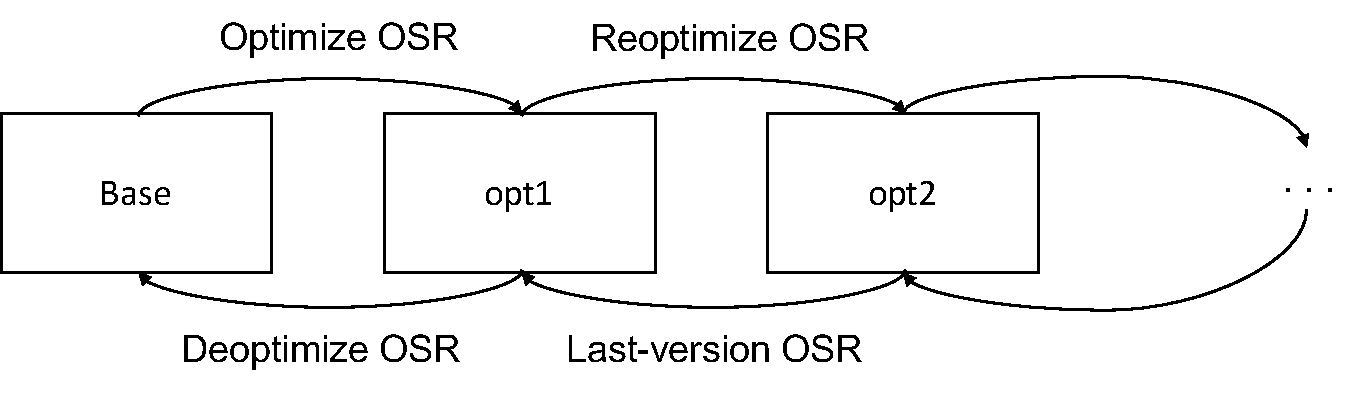
\includegraphics[scale=0.5]{Figures/OSRClassification}
\decoRule
\caption[OSR classification]{OSR classification from CITE}
\label{OSR classification}
\end{figure}

The MCJit library that provides OSR functionalities fit into the regular JIT infrastructure provided by LLVM as described in Figure \ref{MCJitArchitecture} taken from CITE. 
\begin{figure}[h]
\centering
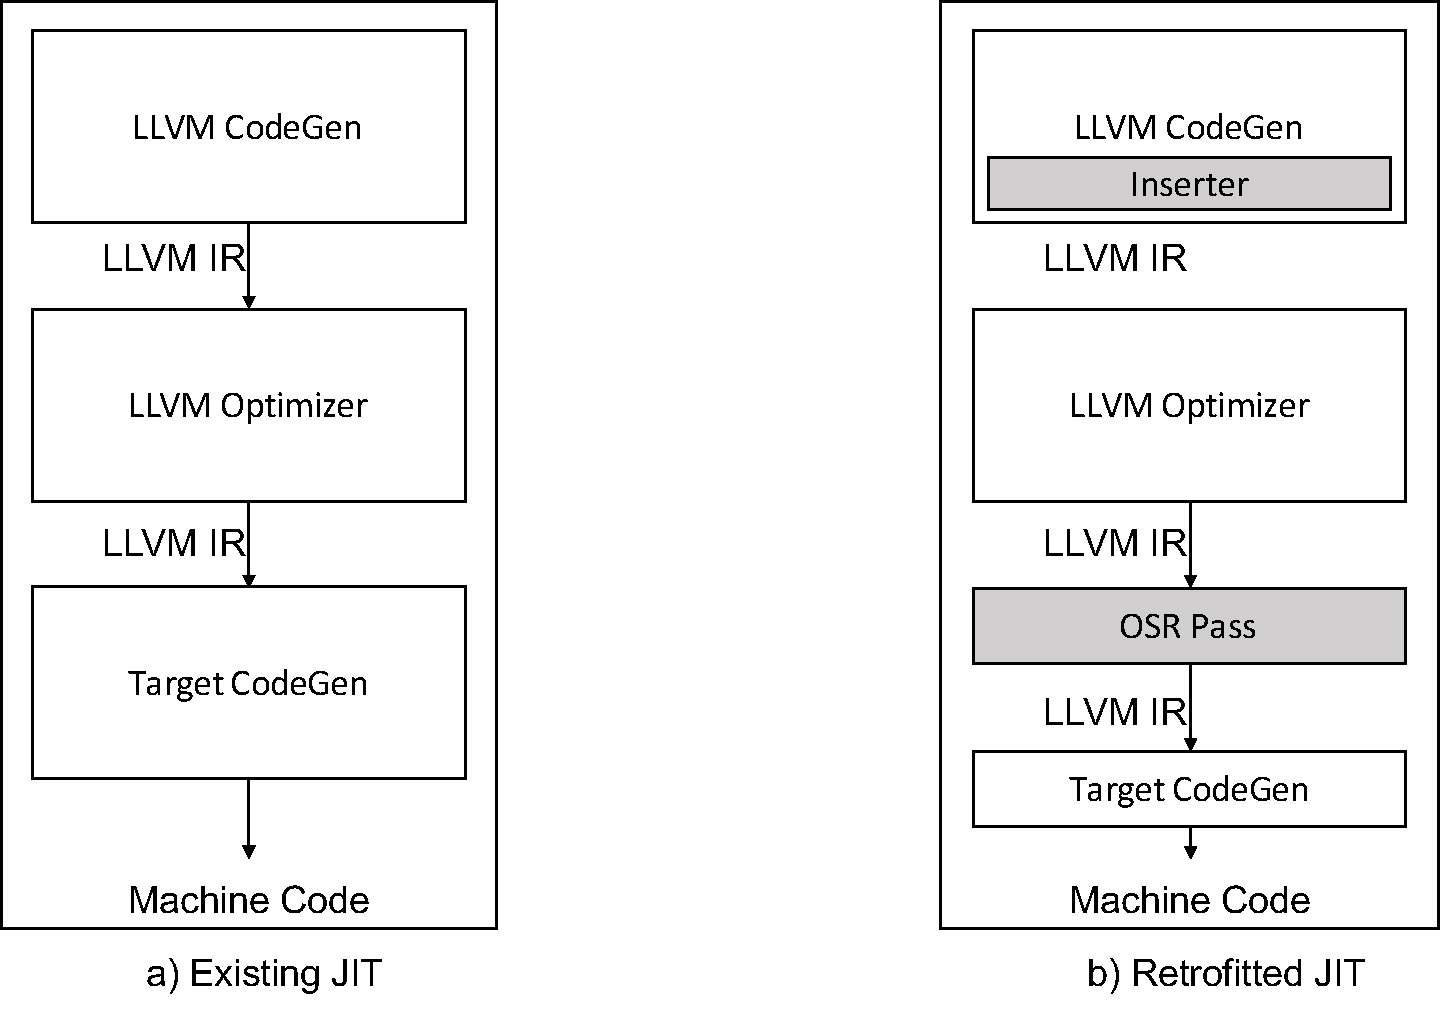
\includegraphics[scale=0.5]{Figures/MCJitArchitecture}
\decoRule
\caption[Retrofitting an existing JIT with OSR support]{Retrofitting an existing JIT with OSR support from CITE}
\label{MCJitArchitecture}
\end{figure}
The left figure is a normal JIT in LLVM. 
The LLVM CodeGen is the front-end of the compiler infrastructure that generates the LLVM IR.
The LLVM Optimizer contains a collection of transformations and optimizations that run on LLVM IR. 
The Target CodeGen outputs the machine code corresponding to the LLVM IR input. 
The MCJit OSR API instruments the LLVM CodeGen to insert OSR points where the OSR transition can be triggered. 
A point is a call to the genOSRSignal function, which takes as arguments a pointer to a code transformer responsible for generating the new version of the function.
The code transformer takes as arguments a pointer to the function that needs to be transformed, and a special OSR label to identify which OSR points triggered the call, if the function contains several ones.
The OSR pass is responsible for instrumenting OSR points with the correct OSR machinery.
The instrumentation saves the live values and creates a descriptor that contains four elements: 
%TODO explain the control version better
\begin{enumerate}
    \item A pointer to the current version of the function. 
    \item A pointer to the control version of the function, i.e., a copy of the old version of the function.
    \item A variable mapping between the original version and the control version.
    \item The set of live variables at the OSR points. 
\end{enumerate}\\

\begin{figure}[h]
\centering
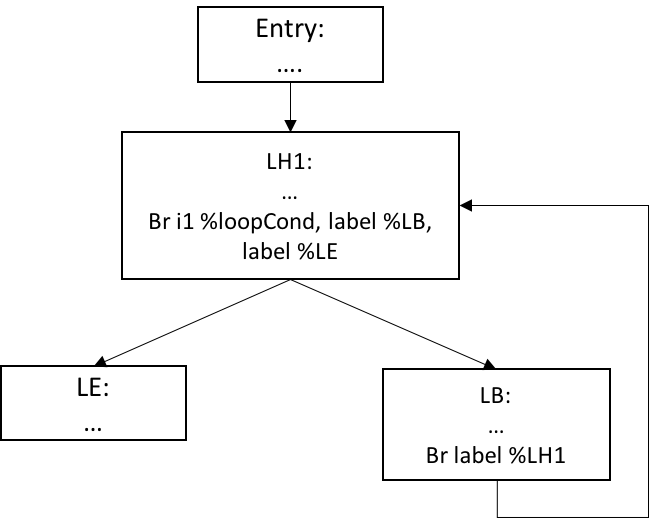
\includegraphics[scale=0.5]{Figures/BaseCFG}
\decoRule
\caption[A CFG of a loop with no OSR point]{A CFG of a loop with no OSR point from CITE.}
\label{BaseCFG}
\end{figure}

\begin{figure}[h]
\centering
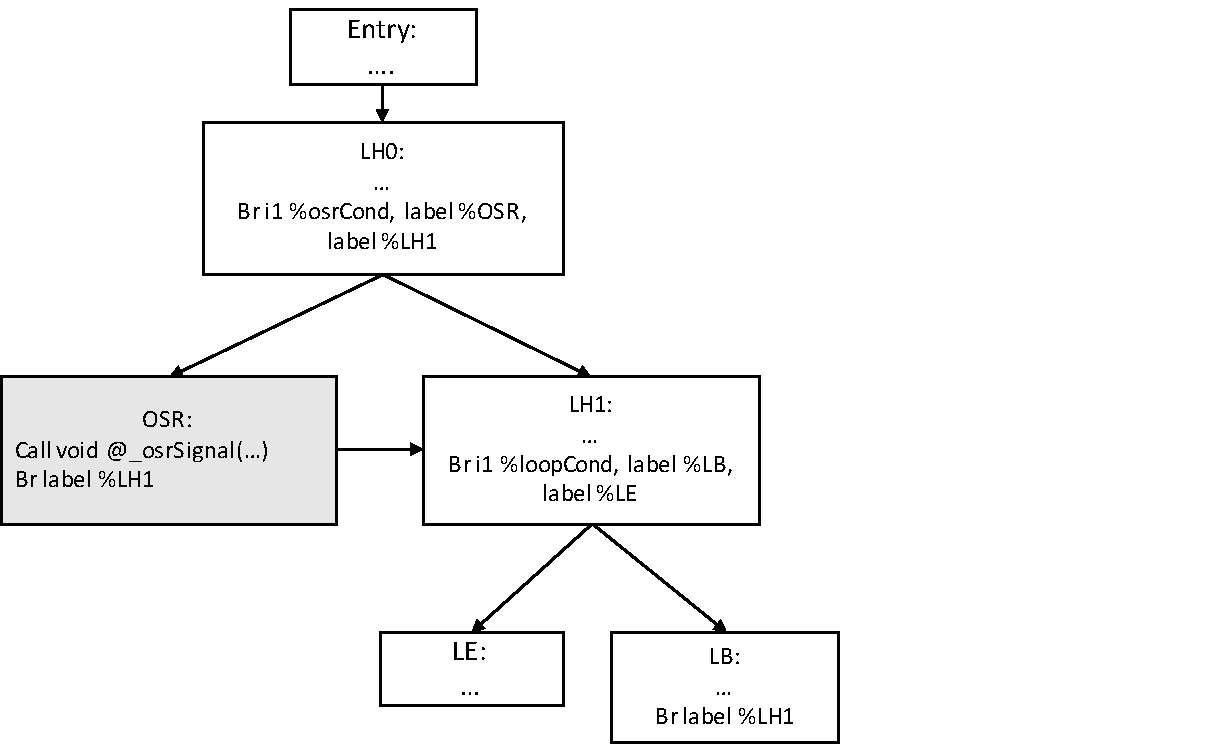
\includegraphics[scale=0.5]{Figures/InsertCFG}
\decoRule
\caption[The CFG of the loop in Figure \ref{BaseCFG}, after inserting an OSR point]{The CFG of the loop in Figure \ref{BaseCFG}, after inserting an OSR point from CITE.}
\label{InsertCFG}
\end{figure}

\begin{figure}[h]
\centering
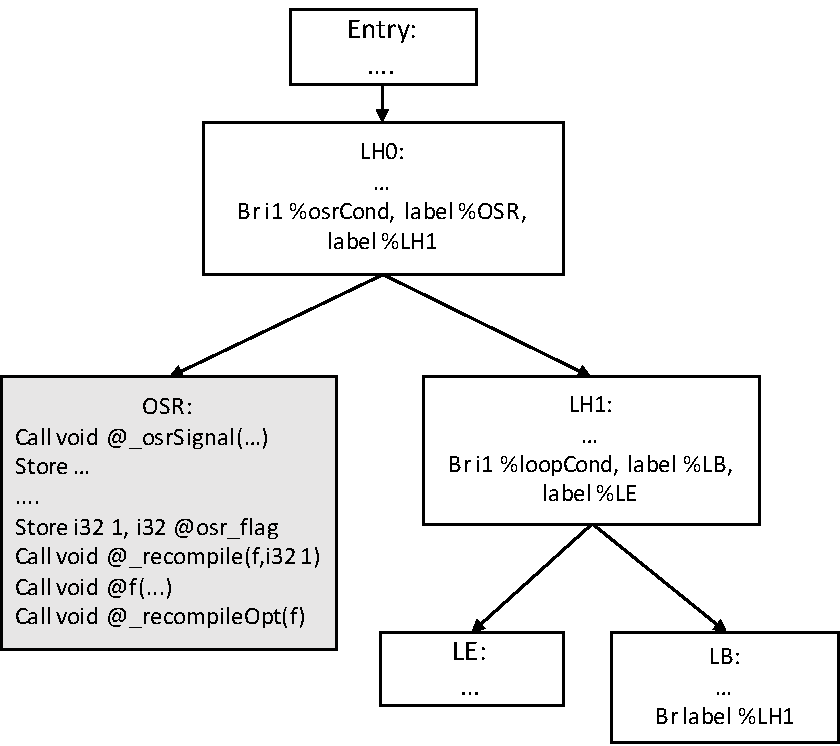
\includegraphics[scale=0.5]{Figures/OSRPassCFG}
\decoRule
\caption[The transformed CFG of the loop in Figure \ref{InsertCFG} after the OSR Pass]{The transformed CFG of the loop in Figure \ref{InsertCFG} after the OSR Pass from CITE.}
\label{OSRPassCFG}
\end{figure}\\

Figures \ref{BaseCFG}, \ref{InsertCFG}, and \ref{OSRPassCFG} give an example of OSR instrumentation at a loop header.
LH1 is the loop header. 
LB is the body of the loop and LE the loop exit. 
Figure \ref{BaseCFG} control flow graph (CFG) is the original CFG. 
Figure \ref{InsertCFG} is the resulting CFG after the Inserter is executed.
Figure \ref{OSRPassCFG}'s CFG corresponds to the result of the OSR pass.
The \textit{recompile} call in the OSR block recompiles \textit{f} using the correct code transformer.
Then \textit{f} calls itself, executing the new version of the function.
This works since the new version lives at the same address as the previous one and is instrumented to jump to the correct instruction, i.e., the one corresponding to the current point at which OSR was triggered.
Figure \ref{FCFG} represents the CFG of \textit{f} before the OSR instrumentation.
Figure \ref{InstFCFG} shows the instrumentation of \textit{f} that enables to jump to the correct instruction in the middle of the function. 
A prolog entry block is inserted at the function header.
This block checks the \textit{OSR flag} to know if an OSR transition is being performed.
If that is the case, it branches to the prolog block that restores the state before resuming the execution at the correct instruction.\\

\begin{figure}[h]
\centering
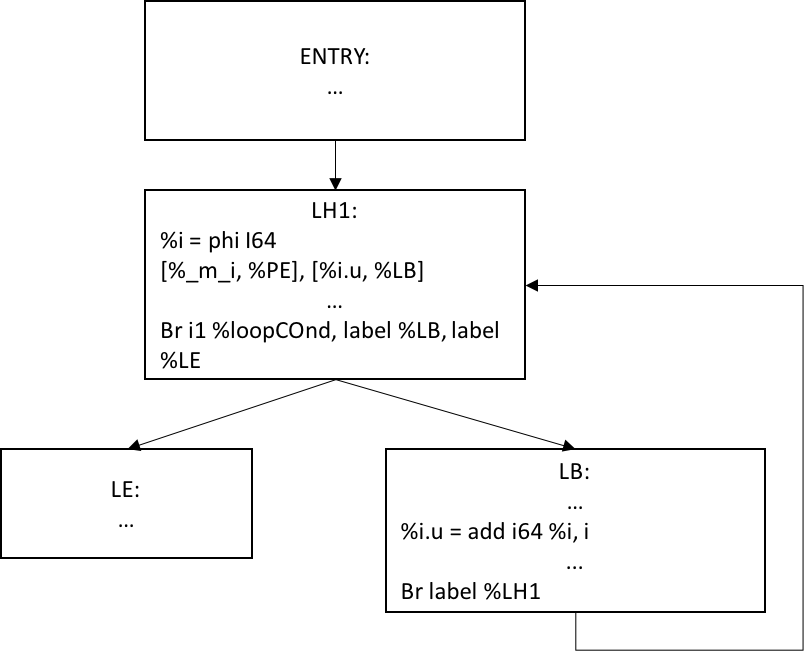
\includegraphics[scale=0.5]{Figures/FCFG}
\decoRule
\caption[A CFG of a running function before inserting the blocks for state recovery]{A CFG of a running function before inserting the blocks for state recovery, from CITE.}
\label{FCFG}
\end{figure}

\begin{figure}[h]
\centering
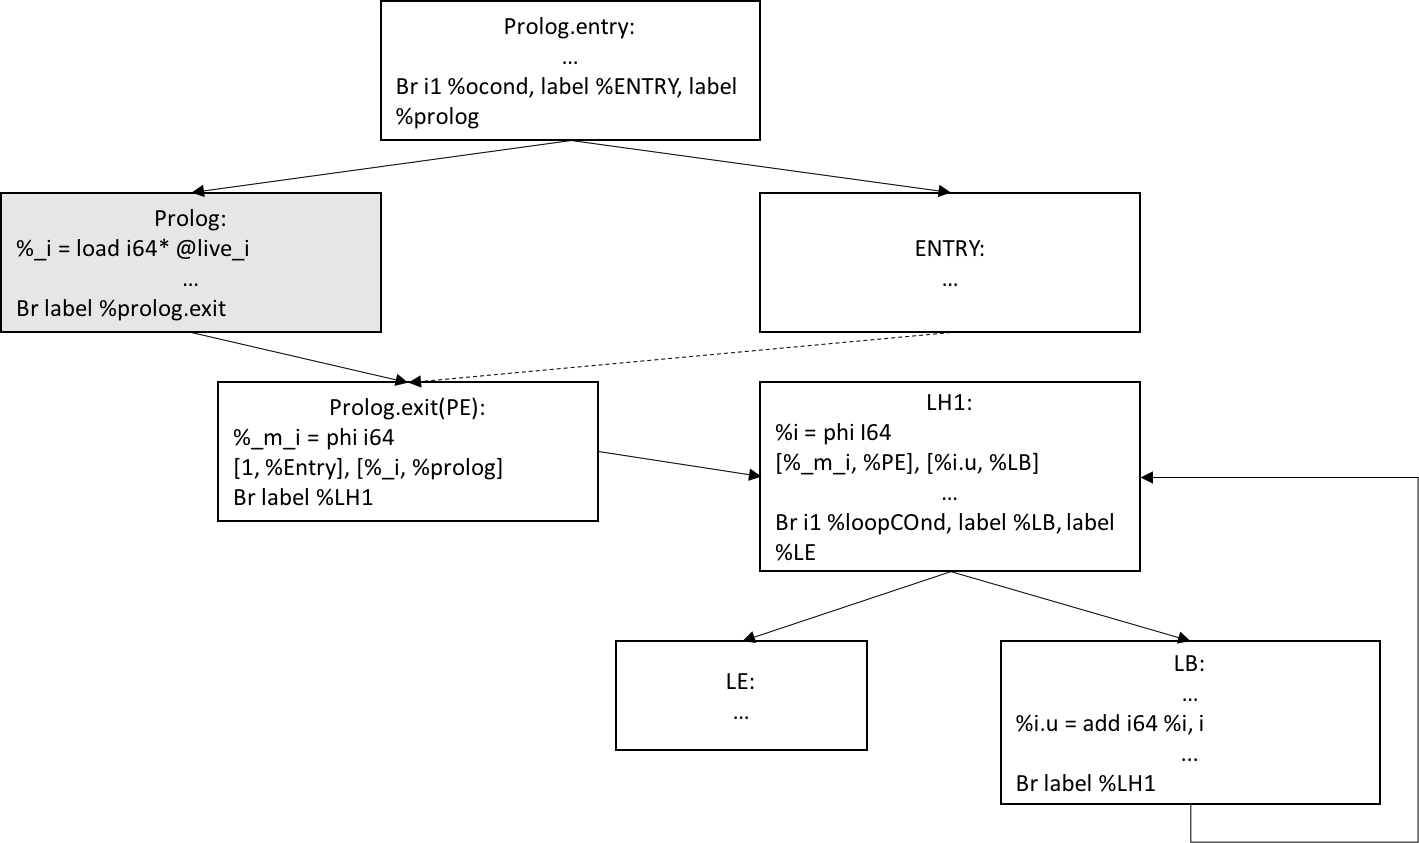
\includegraphics[scale=0.5]{Figures/FOptCFG}
\decoRule
\caption[The CFG of the loop represented in Figure \ref{FCFG} after inserting the state recovery blocks, form CITE.]{The CFG of the loop represented in Figure \ref{FCFG} after inserting the state recovery blocks, form CITE.}
\label{InstFCFG}
\end{figure}\\

%TODO critic of the paper.
The OSR implementation proposed in CITE presents interesting features.
The implementation is done entirely at the LLVM IR, hence making it language-independent.
Furthermore, since the transformation function is provided by the user, any kind of language specific transformation can be used during the OSR.
As a result, MCJit OSR support is an interesting modular OSR library.

On the other hand, this library does not allow to have several versions of the same function, live at the same time.
This restriction can impede the overall performance of the program by extending the scope in which an assumption on which we base the transformation must hold.
For example, a portion of the code, call it \textit{A}, can trigger an OSR, while portion \textit{B} is such that the assumption on which the optimization is based does not hold.
The choice that the user has is to either optimize for A, and deoptimize for B, or to prevent A from optimizing by enlarging the scope in which the assumption is supposed to hold.
None of these solutions is good if \textit{A} and \textit{B} are executed many times, one after the other.
We will either lose a lot of execution time performing OSR, or keep executing \textit{A} without optimization.

In the paper, the deoptimization process is not described. 
It is implied that it relies on the same set of tools provided by the framework as the optimization process, but no example is provided.
As explained in \ref{WhyOSRInteresting}, deoptimization is the most interesting feature of OSR, as it is required to preserve correctness.
Being able to identify where a function should exit is a hard task.
The MCJit library does not provide tools to ease this process and leaves the responsibility to the developer to instrument his functions correctly in order to exit to the correct landing pad.

To the best of our knowledge, MCJit OSR library is not currently used in production or any important project.
As mentioned earlier, WebKit is efficiently integrated in Apple Safari's web browser, which provides useful feedback on its performances.
The lack of usage of MCJit OSR library prevents us from collecting performance results and assess its efficiency.
Furthermore, the experimental evaluation in CITE relies on an example that seems artificial for our use of OSR. 
The case study presents a dynamic inliner that decides to inline a function call if the function is less than 20 basic blocks long, or if it is less than 50 basic blocks long and has an interpreter environment associated with its body. 
This requirement for inlining is one that can be checked statically and, hence, seems a little artificial.\\

\section{A classification summary}
%TODO some kind of sum up and comparison, related to what we had in chapter 2.

%% Chapter 2

\chapter{Related Work} % Main chapter title

\label{Chapter2} % For referencing the chapter elsewhere, use \ref{Chapter2} 

%----------------------------------------------------------------------------------------

% Define some commands to keep the formatting separated from the content 
\newcommand{\keyword}[1]{\textbf{#1}}
\newcommand{\tabhead}[1]{\textbf{#1}}
\newcommand{\code}[1]{\texttt{#1}}
\newcommand{\file}[1]{\texttt{\bfseries#1}}
\newcommand{\option}[1]{\texttt{\itshape#1}}

%----------------------------------------------------------------------------------------

\section{On Stack Replacement, General Principle}

\subsection{Definition \& Overview}
%Replace some portion of code while it is executing 
%Used to optimize code that is running 
%Used to undo an invalid optimization of the code that is running
On-Stack replacement (OSR) is a set of techniques that consist in dynamically transferring the execution, at run time, between different pieces of code.
The action of transferring the execution to another code artefact is called an OSR transition.\\

On-Stack replacement can be viewed, at a high level, as a mechanism that allows to transform the currently executing code, into another version of itself.
This transformation mechanism has been used to allow the bi-directional transition between different levels of code optimizations.
We can therefore reduce it to two main purposes: transforming an executing piece of code into a more optimized version of itself, and undoing transformations that were previously performed.
While similar, these two types of transformation have very different goals.\\

In several virtual machines (CITE PAPERS), some of which will be presented in (REFERENCE), On-Stack replacement has been used to improve the performance of long running functions.
When the VM identifies a piece of code as being "hot", i.e., it hogs the execution, it suspends its execution, recompiles it to a higher level of optimization, and transfers the execution to the newly generated version of the function.
This differs from a simple Just-In-Time (JIT) compiler, since the recompilation takes place during the execution of the function, rather than just before its execution.
%TODO reformulate
However, both techniques rely on run time profiling data to uncover new optimization opportunities.
In this case, OSR is used to improve performance.\\

On-Stack replacement allows a compiler to perform speculative transformations.
Some optimizations rely on assumptions that are not bound to hold during the entire execution of a program.
A simple example is function inlining in an environment where functions can be redefined at any time.
A regular and correct compiler would not allow to inline a function that might be modified during the execution.
The OSR mechanism, on the other hand, enables to perform such an optimization.
Whenever the assumption fails, i.e., the function is redefined, the OSR mechanism will enable to transfer the execution to a corresponding piece of code where the inlining has not been performed.
In this case, OSR is used to preserve correctness.\\

On-Stack replacement is a powerful technique, that can be used to either improve performance, or enable speculative transformations of the code while preserving correctness.
In the next subsection, we present the historical origins of On-Stack replacement and detail its most interesting features.\\ %TODO don't like the word feature
  

\subsection{The origins: SELF debugging}
%SELF needs aggressive optimizations to have reasonable performance. 
%But that prevents from debugging
%Hence OSR enables selective deoptimization at runtime, which provides source level information 
%That makes some optimizations not available since they are hard to undo (e.g. tail %recursion elimination)
%Scope descriptors enable mapping between optimized and unoptimized, enables to keep track %of the position in the virtual call tree etc. (will be detailed). 
%Interrupt points (where, why, how)
%Function invalidation
The SELF programming language is a pure object-oriented programming language.
SELF relies on a pure message-based model of computation that, while enabling high expressiveness and rapid prototyping, impedes the languages performances(CITE from self paper).
Therefore, the language's implementation depends on a set of aggressive optimizations to achieve good performances\cite{holzle1992debugging}.
SELF provides an interactive environment, based on interpreter semantics at compiled-code speed performances.\\

Providing source level code interactive debugging is hard in the presence of optimizations.
Single stepping or obtaining values for certain source level variables might not be possible.
For a language such as SELF, that heavily relies on aggressive optimizations, implementing a source code level debugger requires new techniques.\\

In \citetitle{holzle1992debugging}\cite{holzle1992debugging}, the authors came up with a new mechanism that enables to dynamically de-optimize code at specific interrupt points in order to provide source code level debugging while preserving expected behaviour (CITE from holzle).\\

\citean{holzle1992debugging} present the main challenges encountered to provide debugging behaviours, due to the optimizations performed by the SELF compiler. 
Displaying the stack according to a source-level view is impeded by optimizations such as inlining, register allocation and copy propagation.
For example, when a function is inlined at a call spot, only a single activation frame is visible, while the source level code expects to see two of them.
Figure (FIG), taken from \cite{holzle1992debugging}, provides another example of activations discordances between physical and source-level stacks.
In this figure, the source-level stack contains activations that were inlined by the compiler. For example, the activation B is inlined into A', hence disappearing from the physical stack.\\
\begin{figure}[h]
\centering
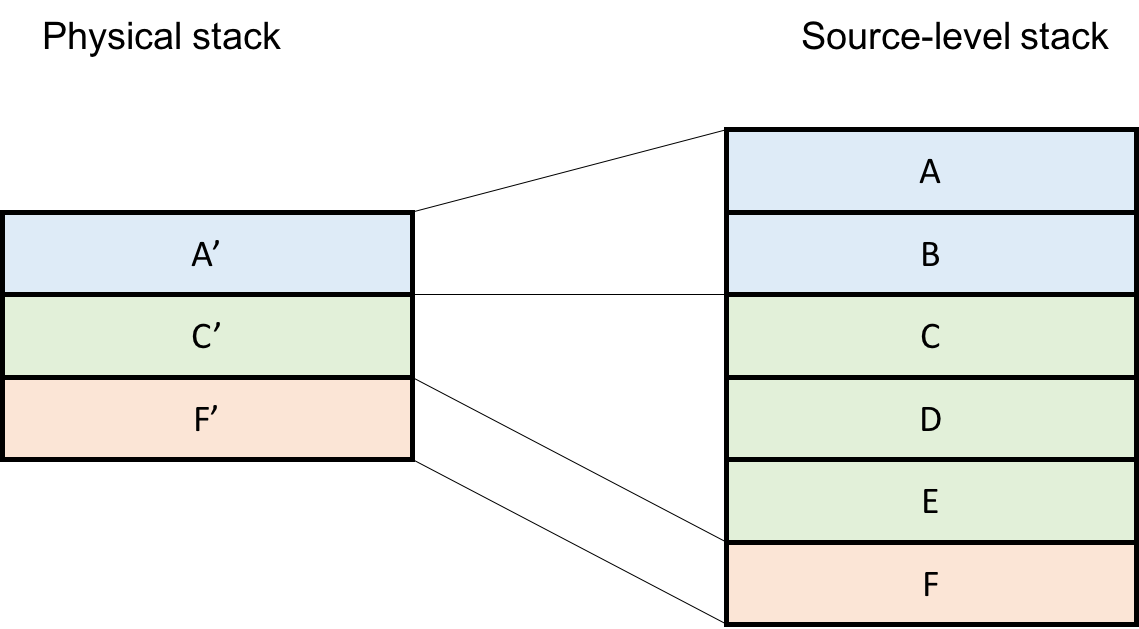
\includegraphics[scale=0.5]{Figures/Figure1}
\decoRule
\caption[physical vs. source-level stacks]{Displaying the stack, figure from \cite{holzle1992debugging}.}
\end{figure}

Single-stepping is another important feature for a debugger. 
It requires to identify and execute the next machine instruction that corresponds to the source operation.
\citean{holzle1992debugging} highlights the impact of code motion and instruction scheduling on the machine instruction layout. 
Such optimizations re-order, merge, intersperse and sometimes delete source-level operations, therefore preventing a straight forward implementation of single-stepping for the debugger.\\

Compiler optimizations prevent dynamic changes from being performed in the debugger.
Holzle(CITE) identifies two separate issues: changing variable values, and modifying procedures (i.e., functions).
To illustrate the first case, Holzle CITE relies on an example where a variable is assigned the sum of two other variables.
The compiler identifies the two variables as being constants and replaces the addition by a direct constant assignment.
A debugger that allows to change variable values at run time would then yield a non correct behaviour if the user modifies one of the two variables. 
This problem does not arise in the case of unoptimized code since the addition is still present. 
For procedures, Holzle CITE describes an example where a function has been inlined by the compiler, but redefined by the user in the debugger.\\

Holzle(CITE) distinguishes two possible states for compiled code: \textit{optimized}, which can be suspended at widely-spaced interrupt points, from which we can reconstruct source-level state, and \textit{unoptimized}, that can be suspended at any source-level operation and is not subjected to any of the above debugging restrictions.\\

In order to deoptimize code on demand, SELF debugger needs to recover the unoptimized state that corresponds to the current optimized one. 
To do so, it relies on a special data structure, called a \textit{scope descriptor}. 
The scope descriptors are generated during compilation for each source-level scope. 
This data structure holds the scope place in the virtual call tree of the physical stack frame and records locations and values of its argument and local variables. 
It further holds locations or value of its subexpressions. Along with the scope descriptor, the compiler generates a mapping between virtual (i.e, scope descriptor and source position within the scope) and physical program counters (PC).
Figure \ref{Holzle2} is taken from CITE and displays a method suspended at two different points. 
At time t1, the stack trace from the debugger displays frame B, hiding the fact that B was inlined inside of A.
At time t2, D is called by C which is called by A, hence, the debugger displays 3 virtual stack frames instead of only one physical frame.\\

\begin{figure}[h]
\centering
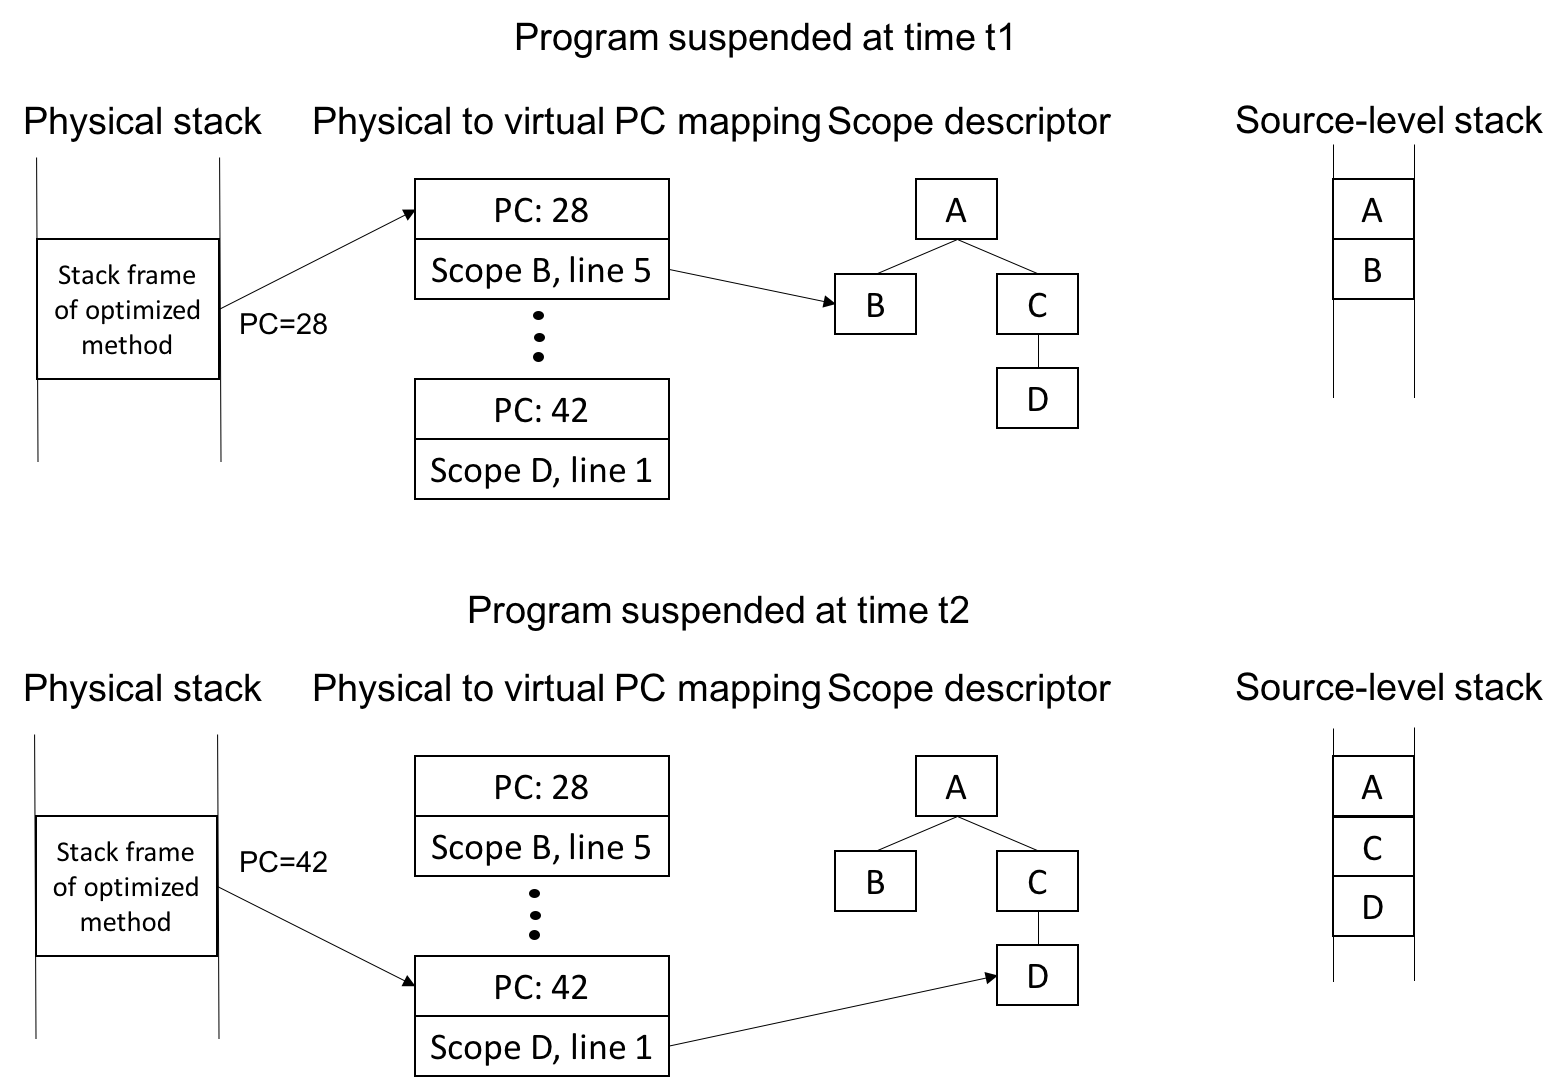
\includegraphics[scale=0.5]{Figures/Figure2}
\decoRule
\caption[Recovering the source-level state]{Recovering the source-level state (from CITE).}
\label{Holzle2}
\end{figure}


The de-optimization process follows 5 steps described in CITE and summed up here:
\begin{enumerate}
    \item Save the physical stack frame and remove it from the run time stack.
    \item Determine the virtual activations in the physical one, the local variables and the virtual PC.
    \item Generate completely unoptimized compiled methods an physical activations for each virtual one.
    \item Find the unique new physical PC for each virtual activation and initialise (e.g., return addresses and frame pointers) the physical activations created in the previous step.
    \item Propagate the values for all elements from the optimized to the unoptimized activations.
\end{enumerate}

Holzle(CITE) also describes \textit{lazy deoptimization}, a technique to deoptimize a stack frame that is not at the current top of the execution stack. 
Lazy deoptimization defers the deoptimization transformation until control is about to return into the frame, hence enabling deoptimization for any frame located on the stack.\\

Deoptimization at any instruction boundary is hard. 
It requires to be able to recover the state at every single point of the program.
Holzle (CITE) relies on a weaker easier restrictions by enabling deoptimization only at certain points called \textit{interrupt points}. 
At an interrupt point, the program state is guaranteed to be consistent. 
The paper (CITE) defines two kinds of interrupt points: method prologues, and backward branches (i.e., end of loop bodies).
Holzle(CITE) therefore estimates the length of the longest code sequence that cannot be interrupted to be a few dozen of instruction, i.e., the average length of a code sequence that does not contain neither a call nor a loop end.
Interrupt points are also inserted at all possible run time errors to allow better debugging of synchronous events such as arithmetic overflow. 
The generated debugging information are needed only at interrupt points, which reduces the space used to support basic debugger operations (as opposed to allowing interrupts at any instruction boundary).\\

Providing a debugger for SELF limits the set of optimizations that the compiler can support, and decreases the performances of the program when the execution is resumed. 
Tail recursion elimination saves stack space by replacing a function call with a goto instruction, while fixing the content of registers.
SELF debugger is unable to reconstruct the stack frames eliminated by this optimization and hence, it is not implemented in the SELF compiler.
More generally, tail call elimination is one important limitation for the SELF debugger.

The debugger slows down the execution when the user decides to resume. 
The execution should proceed at full speed, but some stack frames might have been unoptimized, hence implying that a few frames might run slowly right after resuming execution.\\

\subsection{Why is OSR interesting?}
\label{WhyOSRInteresting}
%The optimization case
     %wait until enough profiling information is gathered to make some new assumptions and improve code quality
    %Some enable to have several specialised versions of the code live at the same time.
    %Chaining OSR means that we can keep optimising the code -> depends on profiler
%The deoptimization case
    %This is the real deal. optimization is not valid without this counter part. 
    %Enables even more agressive code specialisation. Being able to undo means that we can have virtually any assumption and just revert back to a safe version if it fails. 
    %The real difference: optimization is for performance, deoptimazation is for correctness.
    
This section highlights the benefits that On-Stack replacement enables.
We divide them into two separate cases: OSR with regards to optimization, and OSR for deoptimization.\\

On-Stack replacement increases the power of dynamic compilation.
OSR enables to differ compilation further in the future than dynamic compilation techniques such as Just-In time (JIT) compilation.
A function can be recompile while it is executing.
This enables more aggressive adaptative compilation, i.e., by delaying the point in time when the recompilation is performed, OSR enables to gather more information about the current execution profile. These information can then be used to produce higher quality compiled code, displaying better performances.

For dynamic languages, code specialization is the most efficient technique to improve performances (IS THAT TRUE? FIND AND CITE).
Code specialization consists in tuning the code to better fit a particular use of the code, hence yielding better performances.
Specialization can be viewed as a mechanism relying on the versioning of some piece of code.
One of the main challenges is to identify which version better fits the current execution need.
This requires to gather enough profiling information, some of which might not be available until some portion of the code is executed multiple times.

OSR, coupled with an efficient compiler to generate and keep track of specialized functions, enables to uncover new opportunities to fine tune a portion of code.
While techniques like JIT compilation can generate specialized code at a function level, i.e., before the execution of a function, OSR enables to make such tuning while a function is running.
For example, in the case of a long running loop inside a function, JIT techniques would need to wait until the function is called anew to improve its run time performance by recompiling it. 
OSR, on the other hand, gives the compiler the means to make such improvements earlier, hence yielding a better overall performance for the executing program.

OSR is a tool that enables the compiler to recompile and optimize at almost any time during the execution of a program.
A clever compiler can perform iterative recompilation of the code in order to improve the quality of the generated compiled artefact.
OSR enables these iteration steps to be closer to each other and potentially converge to a better solution faster than other dynamic compilation techniques.\\

On-Stack replacement's most interesting feature is deoptimization. 
While optimization enables to increase performance, deoptimization's goal is to preserve correctness of the program that executes.
OSR allows speculative optimizations which, in turn, weakens the requirements for compiled code correctness. 
In other words, the compiler can generate aggressively optimized code. 
Virtually any assumption can be used to generate compiled code and, if the assumption fails, 
OSR enables to revert back to a safe version during the execution.\\

\section{On Stack Replacement \& Virtual Machines}
Virtual machines are privileged environments in which On-Stack replacement can be used to its full power.
As seen in \ref{WhyOSRInteresting}, OSR is as useful as the compiler's profiler is efficient.
A virtual machine (VM) has control over the resources allocation, enables to control the code that is generated by the compiler, and maintains important run time data, state information, and other useful informations about the program being executed.\\

This section presents several examples of VMs that support On-Stack replacement. 
The section is divided into two parts: we first presents several solutions that provide OSR for  the Java programming language, then we briefly introduce LLVM virtual machine, a virtual machine presenting an interesting framework in which we believe On-Stack replacement mechanism should fit.\\ 
\subsection{In Java}
%Java Hotspot 
%Graal 
%Jikes
On-Stack replacement has been used in several virtual machines based on the JVM.
BETTER INTRODUCTION AND TALK ABOUT ALL PAPERS; INCLUDING GRAAL.\\

\subsubsection{Java HotSpot}
The Java HotSpot Performance Engine(CITE web) is a Java virtual machine developed and maintained by Oracle.
The Java HotSpot VM provides features such as a class loader, a bytecode interpreter, Client and Server virtual machines, several garbage collectors, just-in-time compilation and adaptive optimizations.\\

The Java HotSpot Engine supports on-stack replacement in order to provide efficient deoptimization\cite{paleczny2001java}.
When a class loading invalidates an optimization decision, such as a call inlining, the methods relying on this decision need to be deoptimized.
Threads that are executing in a method that needs to be deoptimized are stopped as soon as they reach a safepoint.
The JVM state is recorded as an input of safepoints and procedure calls.
This implies, as a side effect, that the entire JVM state is marked as "live" at a safepoint, hence extending the live range of some values.
The Java HotSpot Engine then extracts the native frame corresponding to this execution trace, and converts it into a byte code interpreter frame.
The execution of the method then continues in the interpreter.
UNCOMMON TRAPS\\

\subsubsection{The Jikes RVM}
The Jikes Research Virtual Machine (RVM)(REF) is an open source, self hosted, i.e., it is entirely implemented in Java, virtual machine for Java programs.
%TODO compile only from Qian.
It provides advanced state-of-the-art features such as dynamic compilation, adaptive optimizations, garbage collection, thread scheduling, and synchronization (CITE).\\

Jikes RVM is an extensible framework in which different On-Stack replacement techniques have been implemented.
%The first
\citean{fink2003design} implemented OSR support in JikesRVM. 
Their implementation relies on JVM scope descriptor, associated to method activation frames.
A scope descriptor contains the thread running the activation, the bytecode index that corresponds to the program counter, values of all local and stack locations, and a reference to the activation's stack frame.
The OSR transition is divided into three steps: 
\begin{enumerate}
    \item Extract the compiler-independent state from a suspended thread. 
    \item Generate the new code for the suspended activation.
    \item Transfer the execution in the suspended thread to a new compiled code.
\end{enumerate}
\citean{fink2003design} generates the target function by compiling a specialized version of the method for each activation that is replaced, as well as a new version for future invocations.
In other words, instead of allowing multiple entry points per function \cite{lameed2013modular, paleczny2001java}, this JikesRVM OSR implementation generates a specialized version of the target function that has only one entry point, corresponding to the instruction from which the OSR transition was triggered.
Each such method contains a special \textit{prologue}, responsible for saving values into locals and loading values on the stack.
OSR transitions can be taken at special points, called \textit{OSR points}, introduced by the optimizing compiler and that correspond to points where the running activation may be interrupted.
The implementation makes a distinction between unconditional and conditional OSR points.
An OSR point is implemented as call that takes all live variables as arguments. 
This constraints some optimizations such as dead code elimination, load elimination, store elimination and code motion by extending the liveness scope of some variables.
An OSR point transfers control to an exit block, i.e., it can be viewed as a non-return call.\\

\citean{soman2006efficient} proposed a general-purpose OSR mechanism, for JikesRVM, that presents less restrictions for compiler optimizations than the previous approach, while decoupling the OSR implementation from the optimization process.
They extend the previous OSR implementation\cite{fink2003design} to enable OSR transition at, and accross points at which the execution can be suspended.
In order to do so, they rely on a special data structure called a \textit{variable map}(VARMAP).
A VARMAP is associated with each method, and consists in a list of thread-switching points and their live variables.
When the compiler performs optimizations, the VARMAP is updated accordingly.
Once the compilation completes, the VARMAP is compressed into a compressed map that contains an entry for each OSR point present in the method. EXPAND ON HOW OSR IS PERFORMED.
\citean{soman2006efficient} also propose an alternative lazy triggering of on-stack replacement.
Lazy triggering consists in taking an OSR transition due to events in the environment, i.e., events triggered by the runtime. 
Whenever the runtime deems an assumption invalide, it invokes a helper function called \textit{OSR helper} that either patches the code of the executing methods to call the OSR process, or it modifies return addresses of the callees of the method to be replaced to point to the OSR helper.
When a callee returns, the OSR helper creates a new stack frame with the state extracted from the specialized method's stack and saves all of the specialized method registers into its stack frame. 
The return address of the OSR helper points to the current instruction in the specialized code, which is then used during OSR to identify the location to resume the execution in the new version of the method.
Lazy triggering improves the code efficiency by avoiding the extra cost of guards evaluations.  



\subsection{LLVM}
%What is LLVM? 
    %Some description of LLVM, putting the emphasis on the fact that it enables to generate native code from LLVM IR, and that many languages have an LLVM compiler (e.g. R, Ruby, Python, Matlab etc.) 
    %Provides tools and mechanism that we can reuse (e.g. low level optimizations, passes on the code etc.) 
%Why OSR on LLVM? 
    %General technique that can be profitable to several languages. 
    %Don’t need to worry about static optimizations 
    %Get portability for free
    %Examples: WebKit & McJit
\subsubsection{LLVM, formerly called Low Level Virtual Machine}
%TODO cite the llvm paper?
LLVM is a compiler infrastructure providing a set of reusable libraries.
LLVM provides the middle layers of a compiler system and a large set of optimizations for compile-time, link-time, run-time, and idle-time for arbitrary programming languages.
These optimizations are performed on an intermediate representation (IR) of the code and yield an optimized IR.
The LLVM framework also provides tools to convert and link code into machine dependent assembly code for a specific target platform.
LLVM supports several instruction sets including ARM, MIPS, AMD TeraScale, and x86/x86-64(CITE?).\\

The LLVM intermediary representation is a language-independent set of instructions that also provides a type system.
The LLVM IR is in static single assignment form (SSA), which requires every variable every variable to be defined before it is used and assigned exactly once. 
SSA enables or improves several compiler optimizations among which constant propagation, value range propagation, sparse conditional constant propagation, dead code elimination, global value numbering, partial redundancy elimination, strength reduction and register allocation.
The SSA requirement for variables to be assigned only once requires a special mechanism, called a $\phi$-node, one a value depends on which control flow branch was executed before reaching the current variable definition.
Figure \ref{SSA example} provides an example where we have to choose between two possible values for a variable after the merging of two control flow branches.

\begin{figure}[h]
\centering
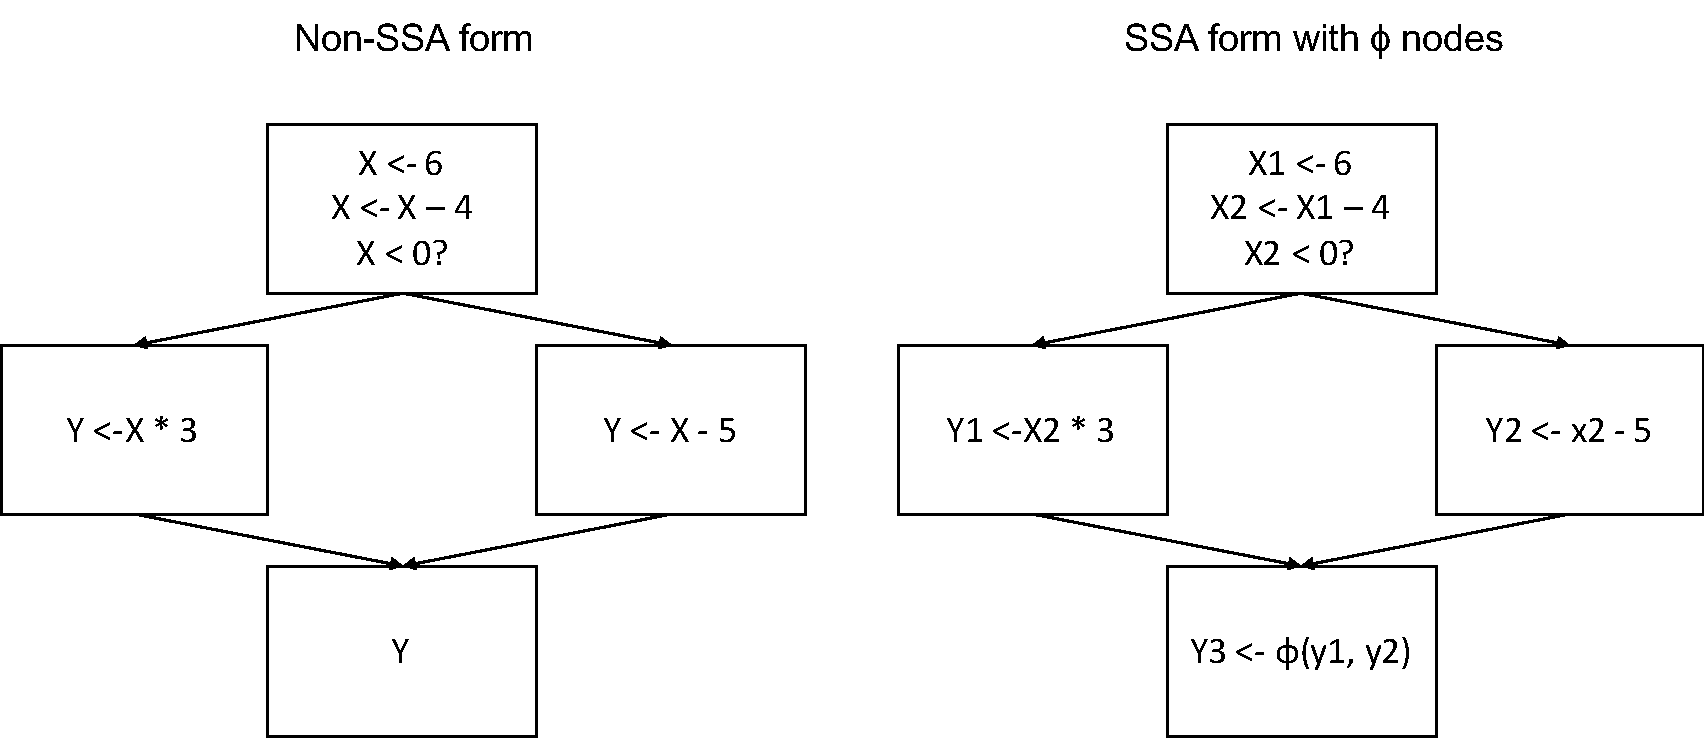
\includegraphics[scale=0.5]{Figures/SSAForm}
\decoRule
\caption[SSA example]{Example of $\phi$-node in SSA form.}
\label{SSA example}
\end{figure}

%TODO exhaustive basic types?
The LLVM IR type system provides basic types (e.g., integers, floats), and five derived types: pointers, arrays, vectors, structures, and functions.
Any type construct can then be represented as a combination of these types.\\

%TODO reformulate/restructure this §
The LLVM framework is a versatile tool that enables to implement many programming languages paradigms.
LLVM compilers exist for several mainstream/popular languages such as Java, Python, Objective-C, and Ruby have an LLVM compiler.
Other languages, like Haskell, Scala, Swift, Rust, Ada, and Fortran also have an LLVM compiler implementation.
LLVM basic types enable to support object-oriented languages, such as Java and Python, dynamically typed languages like R or statically typed like Scala.
LLVM also enables to model functional languages such as Haskell, as well as imperative ones. 
Furthermore, it supports reflection and, thanks to dynamic linking, modular languages (e.g., Haskell).
The tools provided enable static compilation as well as dynamic compilation techniques such as Just-In-Time compilation (JIT).\\

\subsubsection{Why On-Stack replacement in LLVM is interesting}
On-Stack replacement high-level mechanism is language-independent.
Therefore, implementing OSR as a clean modular addition to LLVM would enable developers to leverage this feature in many programming languages, without requiring them to write a new compiler from scratch.
Furthermore, as explained in \ref{WhyOSRInteresting}, OSR is a useful tool for dynamic and adaptative optimizations.
LLVM already provides implementations for many compiler optimizations(CITE) and tools to allow dynamic recompilation of code.
Developers can therefore focus on language specific challenges, such as efficient profilers and new speculative systems, rather than on the optimizations and OSR implementations.

Implementing OSR for LLVM not only serves several languages, but also allows to provide a solution for several target platforms.
As explained previously, LLVM supports several instructions sets corresponding to different architectures.
By implementing OSR in LLVM, we get portability among these platforms for free.\\


\subsubsection{Examples of OSR implementation in LLVM}

OSR has been implemented in LLVM in several projects, such as the WebKit web browser engine and the MCJit project.
In WebKit, OSR and LLVM are part of the four-tier architecture compiler for JavaScript.
The Fourth-Tier LLVM (FTL) is an LLVM-based Just-In-Time compiler.
The WebKit run-time compilation flow is described by Figure \ref{FTL}.\\
\begin{figure}[h]
\centering
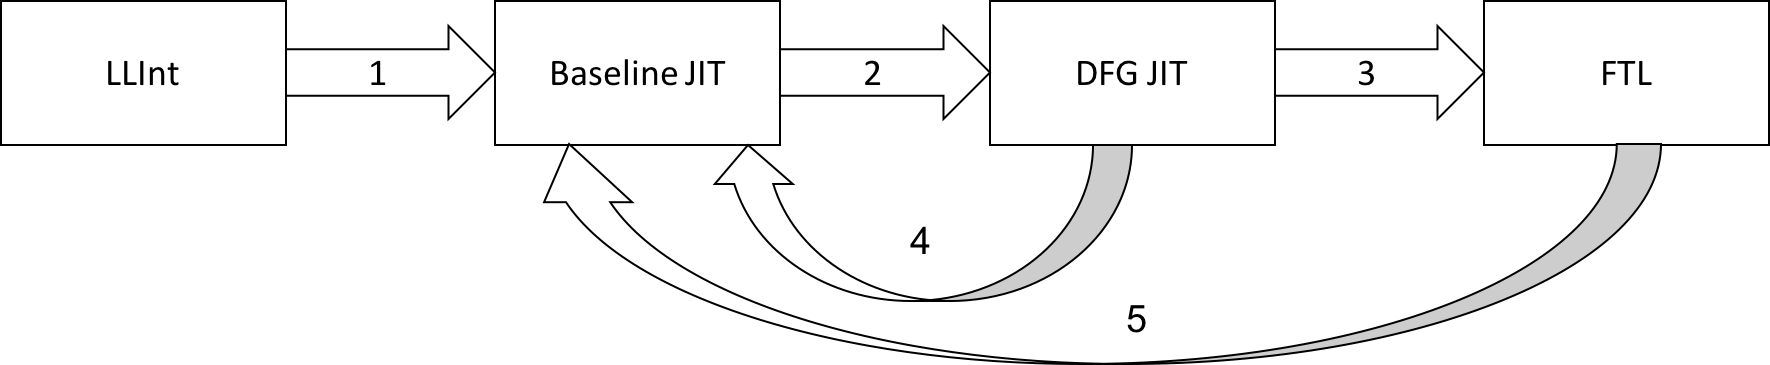
\includegraphics[scale=0.5]{Figures/FTL}
\decoRule
\caption[The WebKit FTL]{The WebKit Four-tier optimization flow.}
\label{FTL}
\end{figure}
 
Forward arrows represent \textit{OSR entries}, i.e., a transformation that yields a more optimized version of the code at run-time.
Backward arrows correspond to \textit{OSR exits}, i.e., a transformation that yields a less optimized version of the code at run-time.
The low level interpreter (LLInt) is used for low latency start up.
The baseline JIT generates WebKit bytecode with no optimization enabled.
The transition from the first tier to the second one happens when a statement is executed more than a hundred times or a function is called more than six times.
The data flow graph (DFG) JIT is triggered when a statement executes more than a thousand times or a function is called more than sixty-six times.
The FTL tier relies on LLVM machine code optimizations to generate a fast version of portions of the code.
In order to hide the costs of the translation to LLVM IR and its compilation time, the FTL is triggered only for long running portions of the code that are currently executing.
There are two kinds of transitions in WebKit: the ones contained entirely inside the WebKit framework (i.e., transitions 1,2 \& 4 in Figure \ref{FTL}), and the ones that involve LLVM (i.e., 3 \& 5 in Figure \ref{FTL}).\\

Transitions to and from LLVM are hard. 
There is no control over the stack layout or the optimized code produced by LLVM.
In the case of transition 3, a different LLVM version is generated for each entry point that the framework desires to have inside this function.
In WebKit, such entry points are located at loop headers. 
This choice makes sense with regard to the condition to enter the FTL, i.e., transition 3 is taken for long running portions of code that could be improved thanks to LLVM low level optimizations.
WebKit has to generate a different version for each entry points for two main reasons: LLVM allows only single entry points to functions (going around this limitation would require to modify LLVM IR and implementation), and instrumenting a function with several entry points would impact on the quality and performance of the generated native code by extending the code's length and restricting code motion.\\

Performing transition 3 requires to get the current state of execution and identify the entry point corresponding to the current instruction being executed.
The DFG dumps its state into a scratch buffer.
An LLVM function with the correct entry point is then generated, and instrumented such that its first block loads the content of the scratch buffer and correctly reconstructs the state.
The mapping between the DFG IR nodes and the LLVM IR values is straight forward since both IR's are in SSA.
A special data structure, called a Stackmap, enables to keep the mapping between LLVM values and registers/spill-slots.\\

Transition 5 is harder as it requires to extract the execution state from LLVM.
WebKit has two different mechanisms to enables OSR exits: the exit thunk and the invalidation points.
In the first case, WebKit introduces exit branches at OSR exit points.
The branch is guarded by an OSR exit condition and is a no-return tail call to a special function that takes all the live non-constant and not accounted for bytecode values.
The second mechanism enables to remove the guard.
Since we assume that the portion of code that is instrumented is executed a lot of times, the cost of testing the condition can have a great impact on the overall execution time.
This mechanism relies on a special LLVM intrinsics, namely patchpoints and stackmap shadow bytes.
A patchpoint enables to reserve some extra space in the code, filled with nop sleds. 
When the WebKit framework detects that an exit should be taken, it overwrites the nop sleds with the correct function call to perform the OSR exit.
This breaks the optimized version of the code which cannot be re-used later on and must be collected.
The stackmap shadow bytes improves on this technique by allowing to directly overwrite the code, without having any nop sled generated before hand.

WebKit is a project that heavily, and successfully relies on OSR to improve performances.
The web browser engine is used in Apple Web browser Safari and enables a net improvement of performances why proving to be reliable(CITE?).
Although successful, it does not provide a general and reusable framework for OSR in LLVM that other projects could reuse.\\

The MCJIT OSR support(CITE) is an attempt at providing an OSR library compatible with the standard LLVM implementation.
Lameed \& Hendren claim to have come up with a clean modular, and re-usable technique completely defined at the LLVM IR level and compatible with the standard LLVM distribution.
There implementation answers to five challenges, listed in the paper CITE and that we reproduce here:\\ 

\begin{enumerate}
    \item Identifying correct interrupt points and using the current LLVM IR to represent them.
    \item Using the LLVM tools to correctly transform the IR while preserving a correct control flow graph. 
    \item Making a new version of a function available at the same address as the old one.
    \item Providing a clean API for the OSR library, that is compatible with LLVM's inlining capabilities.
    \item Integrating OSR without modifying the LLVM installation.
\end{enumerate}

The paper (CITE) claims to support optimization and re-optimization, as well as de-optimization by going back to the previous version of the function.
Figure \ref{OSR classification} shows that this feature only allows single-steps to be taken, i.e., the OSR library implemented in CITE does not seem to allow to skip intermediary versions.\\

\begin{figure}[h]
\centering
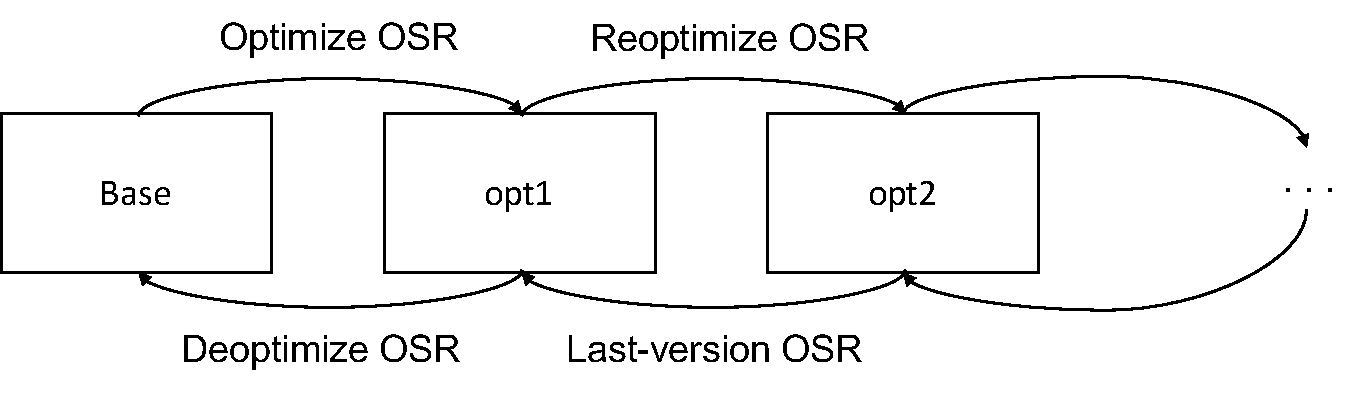
\includegraphics[scale=0.5]{Figures/OSRClassification}
\decoRule
\caption[OSR classification]{OSR classification from CITE}
\label{OSR classification}
\end{figure}

The MCJit library that provides OSR functionalities fit into the regular JIT infrastructure provided by LLVM as described in Figure \ref{MCJitArchitecture} taken from CITE. 
\begin{figure}[h]
\centering
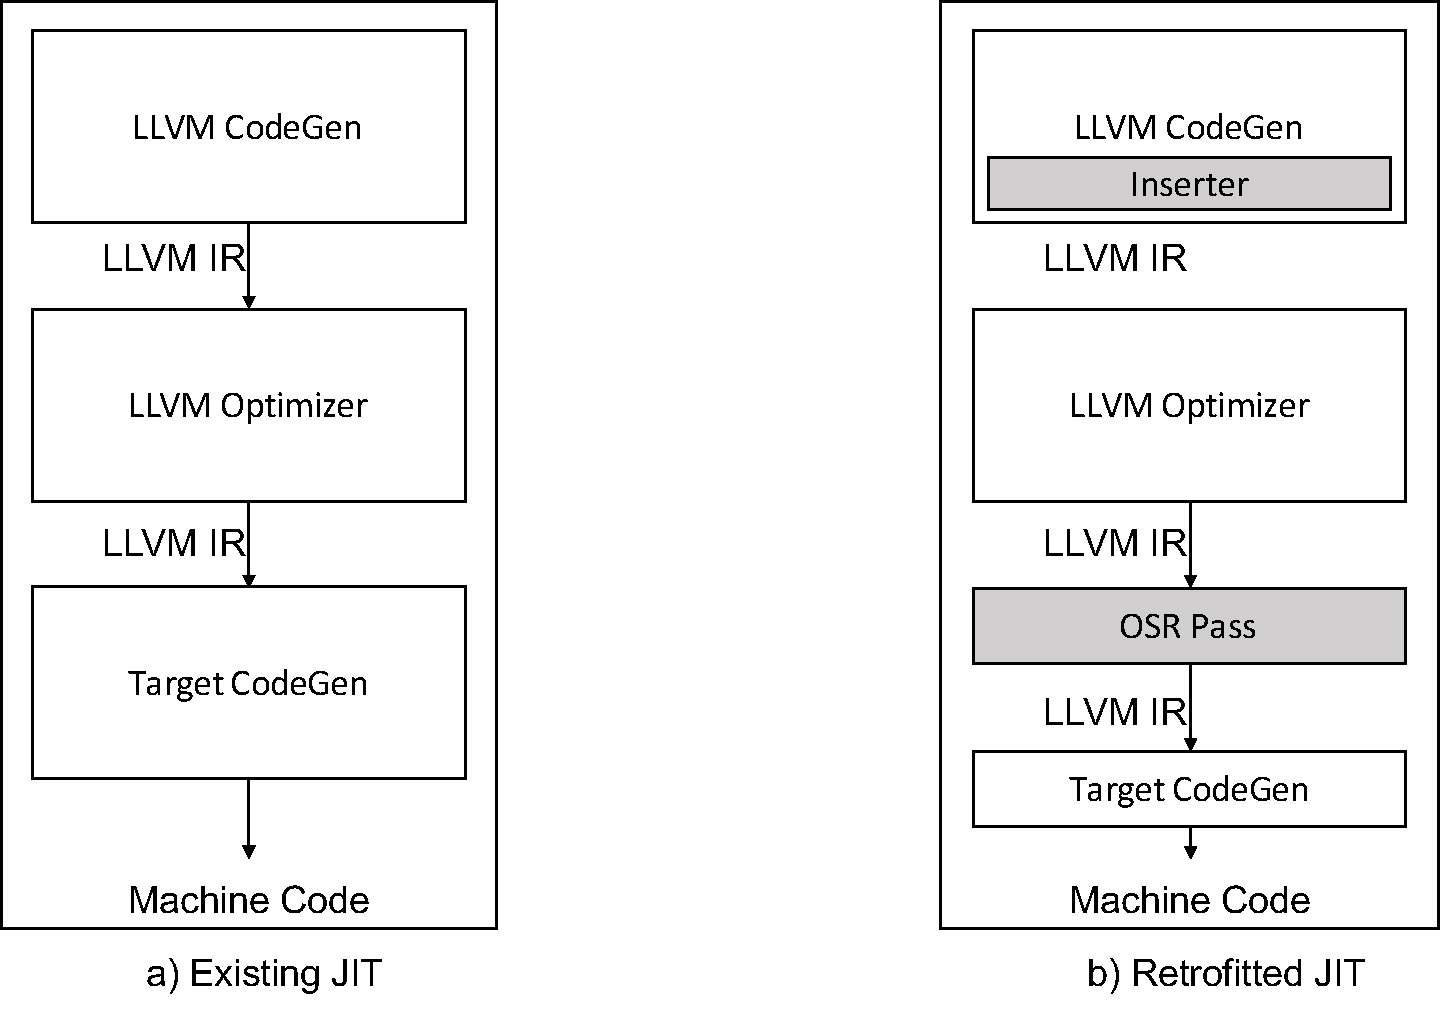
\includegraphics[scale=0.5]{Figures/MCJitArchitecture}
\decoRule
\caption[Retrofitting an existing JIT with OSR support]{Retrofitting an existing JIT with OSR support from CITE}
\label{MCJitArchitecture}
\end{figure}
The left figure is a normal JIT in LLVM. 
The LLVM CodeGen is the front-end of the compiler infrastructure that generates the LLVM IR.
The LLVM Optimizer contains a collection of transformations and optimizations that run on LLVM IR. 
The Target CodeGen outputs the machine code corresponding to the LLVM IR input. 
The MCJit OSR API instruments the LLVM CodeGen to insert OSR points where the OSR transition can be triggered. 
A point is a call to the genOSRSignal function, which takes as arguments a pointer to a code transformer responsible for generating the new version of the function.
The code transformer takes as arguments a pointer to the function that needs to be transformed, and a special OSR label to identify which OSR points triggered the call, if the function contains several ones.
The OSR pass is responsible for instrumenting OSR points with the correct OSR machinery.
The instrumentation saves the live values and creates a descriptor that contains four elements: 
%TODO explain the control version better
\begin{enumerate}
    \item A pointer to the current version of the function. 
    \item A pointer to the control version of the function, i.e., a copy of the old version of the function.
    \item A variable mapping between the original version and the control version.
    \item The set of live variables at the OSR points. 
\end{enumerate}\\

\begin{figure}[h]
\centering
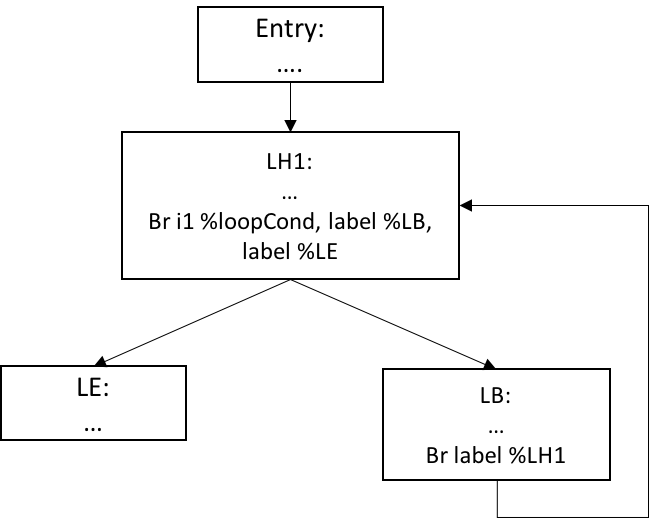
\includegraphics[scale=0.5]{Figures/BaseCFG}
\decoRule
\caption[A CFG of a loop with no OSR point]{A CFG of a loop with no OSR point from CITE.}
\label{BaseCFG}
\end{figure}

\begin{figure}[h]
\centering
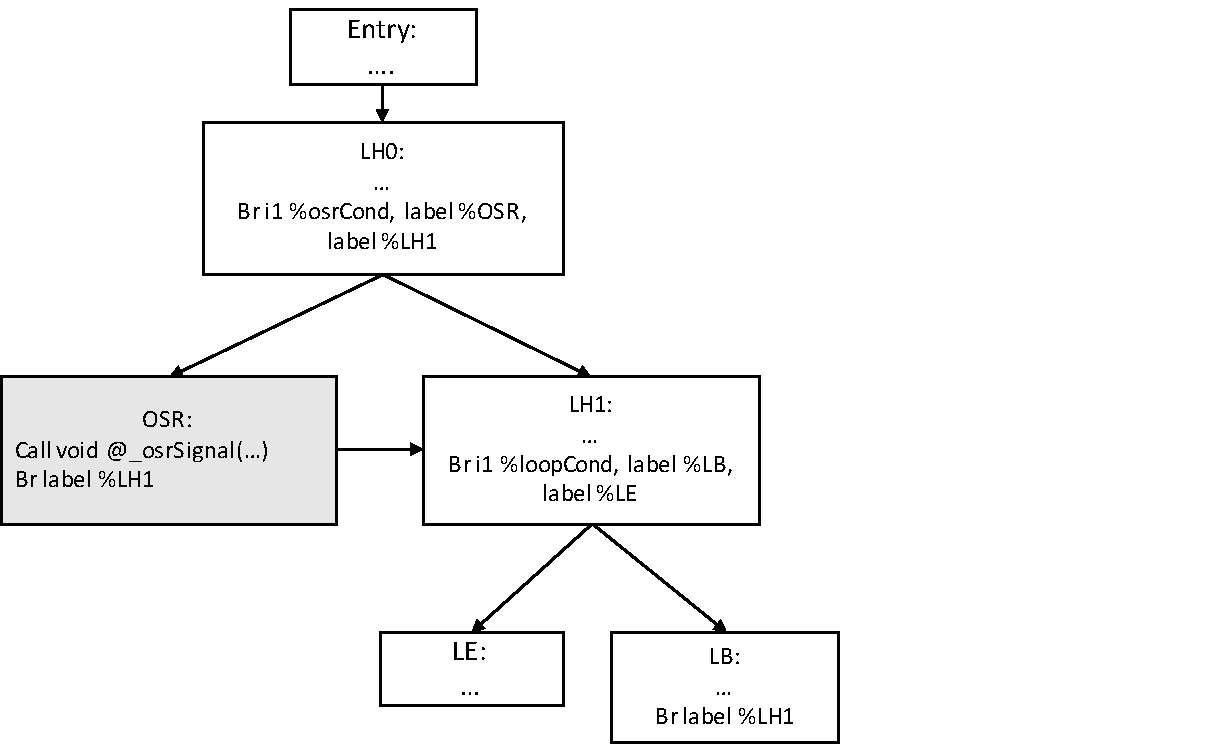
\includegraphics[scale=0.5]{Figures/InsertCFG}
\decoRule
\caption[The CFG of the loop in Figure \ref{BaseCFG}, after inserting an OSR point]{The CFG of the loop in Figure \ref{BaseCFG}, after inserting an OSR point from CITE.}
\label{InsertCFG}
\end{figure}

\begin{figure}[h]
\centering
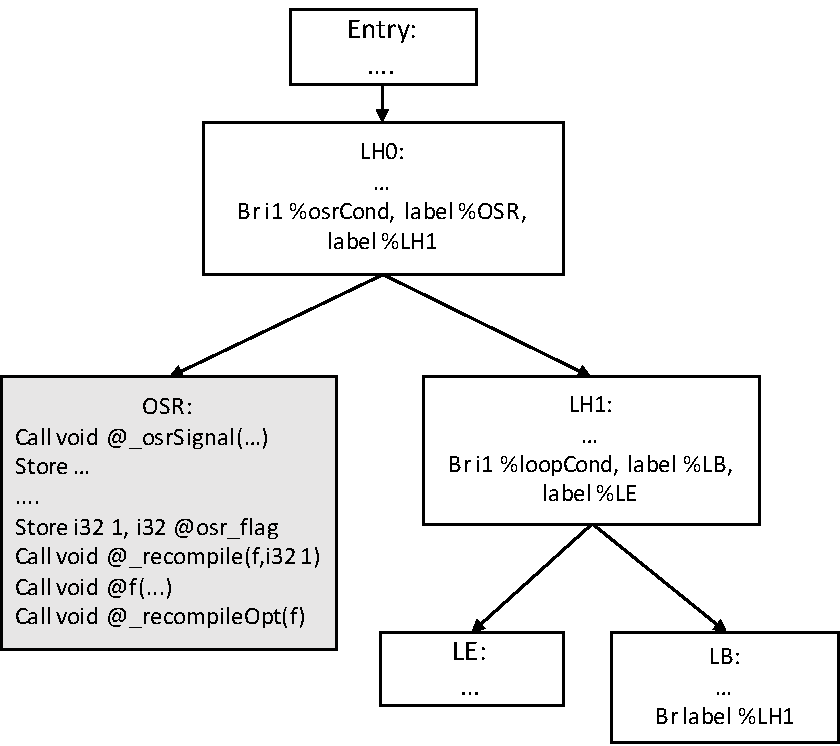
\includegraphics[scale=0.5]{Figures/OSRPassCFG}
\decoRule
\caption[The transformed CFG of the loop in Figure \ref{InsertCFG} after the OSR Pass]{The transformed CFG of the loop in Figure \ref{InsertCFG} after the OSR Pass from CITE.}
\label{OSRPassCFG}
\end{figure}\\

Figures \ref{BaseCFG}, \ref{InsertCFG}, and \ref{OSRPassCFG} give an example of OSR instrumentation at a loop header.
LH1 is the loop header. 
LB is the body of the loop and LE the loop exit. 
Figure \ref{BaseCFG} control flow graph (CFG) is the original CFG. 
Figure \ref{InsertCFG} is the resulting CFG after the Inserter is executed.
Figure \ref{OSRPassCFG}'s CFG corresponds to the result of the OSR pass.
The \textit{recompile} call in the OSR block recompiles \textit{f} using the correct code transformer.
Then \textit{f} calls itself, executing the new version of the function.
This works since the new version lives at the same address as the previous one and is instrumented to jump to the correct instruction, i.e., the one corresponding to the current point at which OSR was triggered.
Figure \ref{FCFG} represents the CFG of \textit{f} before the OSR instrumentation.
Figure \ref{InstFCFG} shows the instrumentation of \textit{f} that enables to jump to the correct instruction in the middle of the function. 
A prolog entry block is inserted at the function header.
This block checks the \textit{OSR flag} to know if an OSR transition is being performed.
If that is the case, it branches to the prolog block that restores the state before resuming the execution at the correct instruction.\\

\begin{figure}[h]
\centering
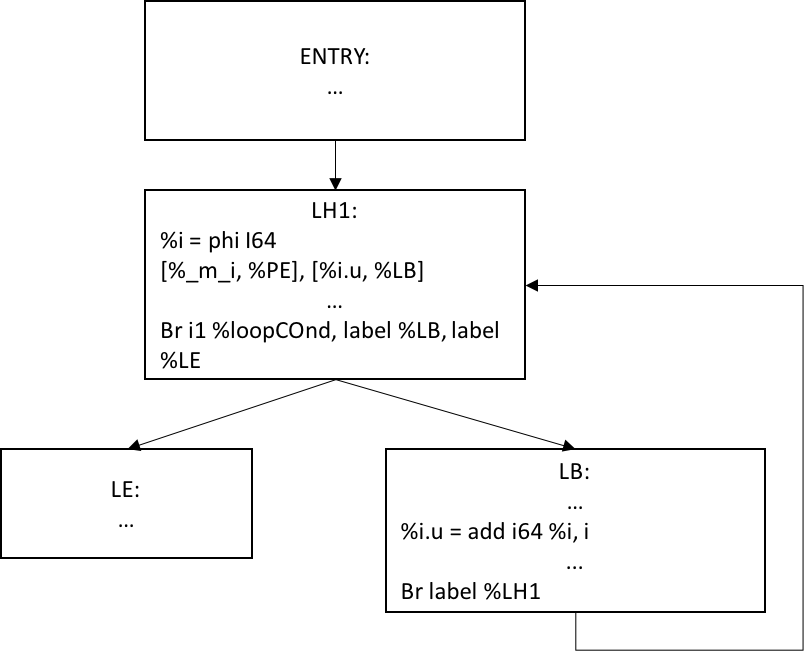
\includegraphics[scale=0.5]{Figures/FCFG}
\decoRule
\caption[A CFG of a running function before inserting the blocks for state recovery]{A CFG of a running function before inserting the blocks for state recovery, from CITE.}
\label{FCFG}
\end{figure}

\begin{figure}[h]
\centering
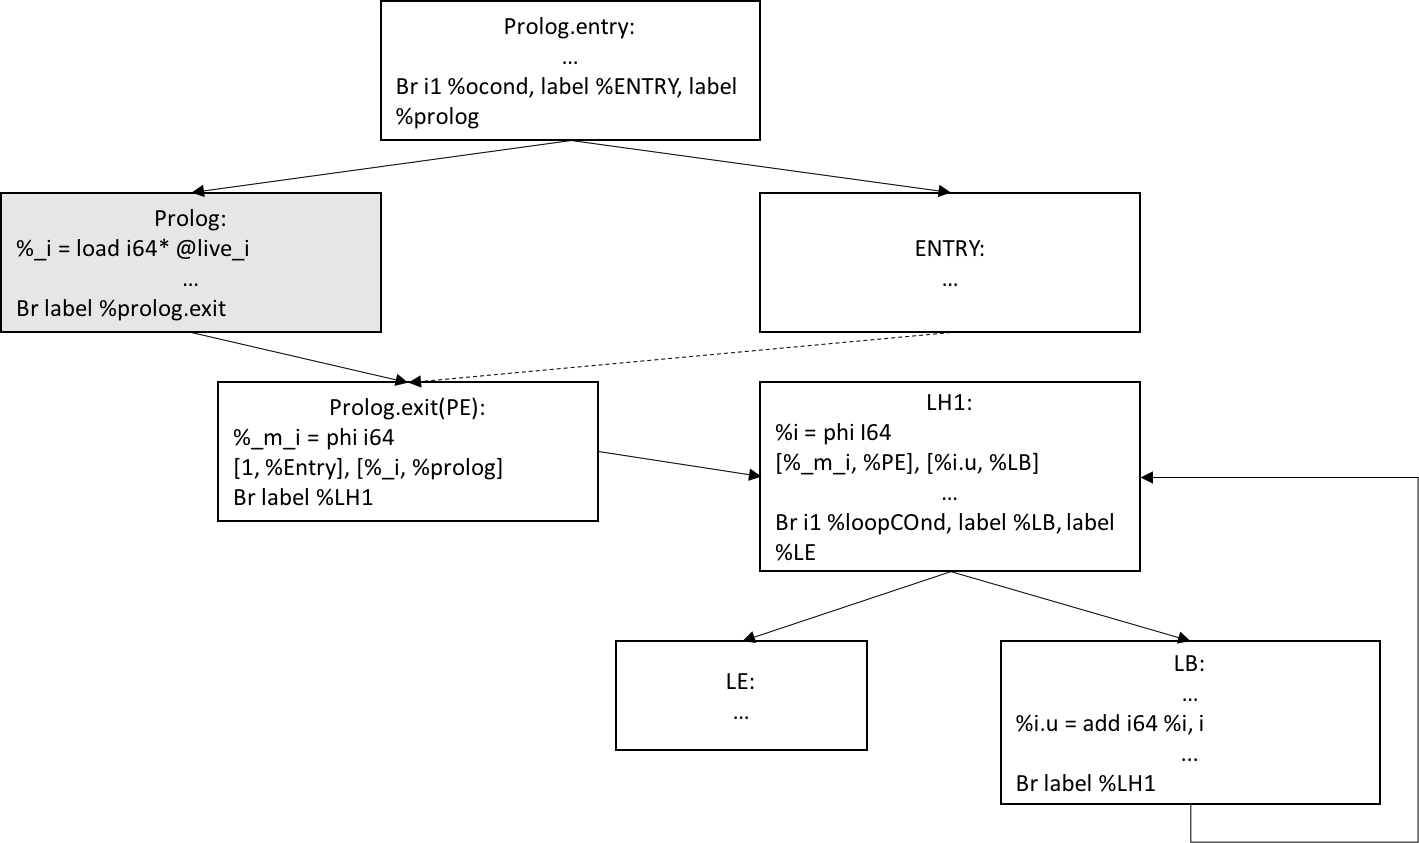
\includegraphics[scale=0.5]{Figures/FOptCFG}
\decoRule
\caption[The CFG of the loop represented in Figure \ref{FCFG} after inserting the state recovery blocks, form CITE.]{The CFG of the loop represented in Figure \ref{FCFG} after inserting the state recovery blocks, form CITE.}
\label{InstFCFG}
\end{figure}\\

%TODO critic of the paper.
The OSR implementation proposed in CITE presents interesting features.
The implementation is done entirely at the LLVM IR, hence making it language-independent.
Furthermore, since the transformation function is provided by the user, any kind of language specific transformation can be used during the OSR.
As a result, MCJit OSR support is an interesting modular OSR library.

On the other hand, this library does not allow to have several versions of the same function, live at the same time.
This restriction can impede the overall performance of the program by extending the scope in which an assumption on which we base the transformation must hold.
For example, a portion of the code, call it \textit{A}, can trigger an OSR, while portion \textit{B} is such that the assumption on which the optimization is based does not hold.
The choice that the user has is to either optimize for A, and deoptimize for B, or to prevent A from optimizing by enlarging the scope in which the assumption is supposed to hold.
None of these solutions is good if \textit{A} and \textit{B} are executed many times, one after the other.
We will either lose a lot of execution time performing OSR, or keep executing \textit{A} without optimization.

In the paper, the deoptimization process is not described. 
It is implied that it relies on the same set of tools provided by the framework as the optimization process, but no example is provided.
As explained in \ref{WhyOSRInteresting}, deoptimization is the most interesting feature of OSR, as it is required to preserve correctness.
Being able to identify where a function should exit is a hard task.
The MCJit library does not provide tools to ease this process and leaves the responsibility to the developer to instrument his functions correctly in order to exit to the correct landing pad.

To the best of our knowledge, MCJit OSR library is not currently used in production or any important project.
As mentioned earlier, WebKit is efficiently integrated in Apple Safari's web browser, which provides useful feedback on its performances.
The lack of usage of MCJit OSR library prevents us from collecting performance results and assess its efficiency.
Furthermore, the experimental evaluation in CITE relies on an example that seems artificial for our use of OSR. 
The case study presents a dynamic inliner that decides to inline a function call if the function is less than 20 basic blocks long, or if it is less than 50 basic blocks long and has an interpreter environment associated with its body. 
This requirement for inlining is one that can be checked statically and, hence, seems a little artificial.\\

\section{A High-Level Description of Existing Solutions}
\subsection{The OSR points}
%TODO do a definition case for that
%Several names for it 
%what it is: a point in the code from which we can suspend the exec and optimize the current version of the code
    %Implies that we need a "safe state”, i.e., we need to be able to find an equivalent point in the optimized version
    %portions of code that don’t have interrupts
    %Too many -> bad Too few -> bad
%Guarded vs Unguarded 
    %Guarding when there is an explicit condition that we can check locally
    %What if global/External event? 
        %Some have a map of such points and fix them whenever an external event happens (citing papers e.g., jikes)
%OSR exits 
    %What to do when the condition fails? 
        %optimization dependent 
        %for external requires to correct every callee return landing spots. 
        %Requires corresponding entry in the unoptimized version
%Examples from existing implementations 
    %MCJIt inserter and instrument passes (need a code transformer + OSR Label)
    %Jikes
The OSR mechanism is enabled at specific instruction boundaries in the user's code.
Depending on the OSR implementation, these points can be sparse, restricted to special points in the control flow, or associated with special framework dependent data.
%TODO not sure next sentence is needed.
This section presents different implementations of such points in the available literature.
In the examples of OSR implementations given so far (CITE SECTIONS), they have been called \textit{interrupt points}(CITE), \textit{OSR entries}, and \textit{OSR exits}(CITE).
In the reminder of this paper, we will refer to such points as \textit{OSR points}, as defined in Definition \ref{OSRPointDefinition}.

\begin{definition}\label{OSRPointDefinition}
An OSR point is a portion of code that belongs to the OSR instrumentation.
It is located at an instruction boundary at which the program can be suspended.
OSR points can correspond to several instructions inserted by the OSR framework and enable to switch the execution from one version of the code to another.
\end{definition}

%TODO continue this part by explaining why we need it to be safe
An OSR point has to be located at a point of the code where the state is \textit{safe}, i.e., points where the state is guaranteed to be consistent.
For example, as explained before, the SELF debugger considers points at method prologues and at the end of loop bodies.
An OSR point must be such that the state of the computation can be extracted and transferred to another version of the code from which we can resume the execution.\\

An OSR point can be guarded or unguarded.
The WebKit OSR framework (CITE) and the Jikes RVM OSR implementation(CITE) distinguish OSR points that are guarded, i.e., there is a boolean condition wrapping the execution of the point, from unguarded ones.
A guarded OSR point is such that the framework has enough information locally to test whether or not an OSR transition should be taken.
While simple to model at a high-level, a guarded OSR points presents the disadvantage of increasing the length of the OSR instrumentation, hence impacting on the overall performance of the program.
As a result, implementations likes WebKit and Jikes RVM OSR provide a second mechanism that we call unguarded OSR points.
In WebKit, an unguarded OSR point is a portion of the code that can be overwritten on some external condition, and hence instrumented to trigger an unconditional transition to another version whenever it is re-written.
It also enables to lazily define the transition, i.e., the instrumentation that enables to jump out of the current version can be added just before being executed.
TALK ABOUT IN JIKES\\

There is a further distinction between OSR points that are responsible for optimising the code, and the ones that are used to unoptimize.
For that, we will use the same terminology as in WebKit and MCJit(CITE).
%TODO reformulate definitions
\begin{definition}\label{OSREntryDefinition}
An OSR entry is an OSR point that enables to replace the current version of the code with one in which we expect to have better performances.
They are used in the optimization process.
\end{definition}

\begin{definition}
An OSR exit is an OSR point that enables to exit the current version of the code when it is invalidated.
OSR exits are responsible for preserving the correctness of the program.
They are used in the deoptimization process.
\end{definition}

CONTINUE

\subsection{The Transition Mechanism}
%The ideal model 
    %Being able to stop execution, save the state, generate a new version, fix the state, replace the instruction pointer and resume.
%The more reasonable case of function calls 
    %Implemented as a function call: return or no return 
    %In SELF: data structures on the side to keep mapping between virtual and physical (might be redundant with 2.1.2)
    %Jikes: the VARMAP that enables to do it virtually at and across OSR points, registers state etc. 
    %MCJit: Saving all live variables, instruments code to jump to correct spot in new version by instrumenting the prolog of the function + executing a special block to fix the state etc. 
    %Rome & Others (to be defined): pass everything as arguments, do a function call and instrument entry point of the function to fix the state and jump to correct continuation point.  

\subsection{Constraints and Limitations}
%Limits the types of optimizations that can be performed (e.g. tail recursion elimination in SELF) 
%Limits code motion + Mechanisms extend variable live range
%Limited spots where we can perform the transition, often limited to function pro/epilogues and loops  
    %Due to the difficulty of finding/ensuring a mapping between optimized and unoptimized otherwise. 
%The space complexity 
    %need to keep additional information around (e.g. variables that were eliminated need to be correctly re-generated when deoptimizing)
    %Instrumentation increases the code

\subsection{Generating on the Fly VS Caching}
%Caching enables to keep several versions around + saves compilation time
%On the fly: we can keep the same address for the function

\subsection{Discussion}
%The proposed classification in MCJit (several optimization, possible deoptimization) 
%The trade off between performance gain and the compilation & instrumentation costs. 
%The paradoxal goal of finding a general technique to aggressively specialise code in particular assumption based circumstances. 
    %By being too general, we actual bring limitations to the implementation 
    %Assumption based optimizations need to be implemented for the OSR mechanism (e.g., mcjit “transformer” method) 
        %How to find a correct API that satisfies every possible optimization that we might want to perform? 
            %Support external event
            %Support guards
%The challenge of code motion 



 
% Chapter 4

\chapter{Deoptimization in RJIT} % Main chapter title

\label{Chapter4} % For referencing the chapter elsewhere, use \ref{Chapter4} 

%----------------------------------------------------------------------------------------

% Define some commands to keep the formatting separated from the content 
\newcommand{\keyword}[1]{\textit{#1}}
\newcommand{\tabhead}[1]{\textbf{#1}}
\newcommand{\code}[1]{\texttt{#1}}
\newcommand{\file}[1]{\texttt{\bfseries#1}}
\newcommand{\option}[1]{\texttt{\itshape#1}}

%----------------------------------------------------------------------------------------
This chapter presents our design to support OSR transitions and OSR deoptimizations in LLVM, and more particularly in the RJIT project.
Our design and implementation is based on OSR Kit\cite{OSRKit, OSRKitGit}, an OSR library for LLVM, implemented by \citean{OSRKit} at the department of Computer, Control, and Management Engineering of the Sapienza University of Rome.
This implementation provides several features of existing techniques, that were never simultaneously supported in a single framework.
It is flexible enough to be used to implement our own model for OSR deoptimization.
We therefore decided to use and extend it, in order to provide OSR deoptimization for R.\\

\section{Overview}
This section presents our goals for this Master Thesis Project and justifies the use of the OSR Kit as the base of our OSR support in RJIT.\\

%TODO MAYBE switch the Justification and the LLVM Library

\subsection{Justification}
%Our goal: OSR deoptimization for R.
    %R has shitty performances
    %need aggressive optimizations
    %Work with the rjit project, so based on LLVM. 
    %Too soon to know what we really want, so need a mechanism as flexible as possible.
%What do we want form OSR Kit? 
    %A transition mechanism
    %An LLVM library that is mostly optimization and language independent.
        %Why? Because we want to work at the LLVM IR level, which is stable.
%Why not from scratch?
    %Reinventing the wheel seems like a waste of time. 
    %Enables to focus on deoptimization case.
    %Enables to test a proper optimization. 
    %Can extend it with new features, can modify it.
The goal of this Master Thesis project is to provide a flexible OSR deoptimization framework in LLVM, and use it to improve performances in RJIT, our LLVM JIT compiler for R.
R is a programming language and software environment for the statistical computing and graphics, developed by the R Foundation for Statistical Computing\cite{RURL}.
Due to SAY WHYYYYYYYYYYYYYYYYYYYYYYYYYY OOOOOHHHHH GOOOOOOODDDDDD WHHHYYYYYYYYYY, R exhibits very poor performances CITE SOMETHING.
The RJIT project strives to improve these performances by providing a LLVM based JIT compiler for R. SAY MORE.
The RJIT compiler is still pretty young, only a few months old.
As a result, we lack FEEDBACK; DONT KNOW EXACTLY HOW TO IMPROVE PERF AND NEED TO EXPERIMENT.
Therefore, we are looking for a flexible and extensible OSR mechanism that enables us to prototype and experiment various solutions, without trapping ourselves into a single model.\\

The OSR Kit library\cite{OSRKit} is a flexible implementation of on-stack replacement instrumentation in LLVM.
The source-code for the library is available on Github\cite{OSRKitGit}, and the library can be used in any LLVM project by simply copy-pasting the OSR Kit files inside of it.
The simple integration, the availability of the source code, and the flexibility of the framework make it a perfect base implementation upon which we can implement our support for OSR deoptimization mechanisms in RJIT.\\

%TODO MORE ABOUT THE FOCUS ON DEOPT.
This master project thesis focuses on the design and implementation of a prototype for OSR deoptimization support in RJIT.
Starting a new OSR transition implementation from scratch requires time.
Using a flexible and modifiable OSR transition library therefore seemed like the goto option.
We do not waste time reimplementing something that already exists, and can therefore put all our efforts into implementing an interesting OSR deoptimization case, testing it, and extending the OSR Kit library with mechanisms that are specific to our needs (Sections \ref{osrForUs} and \ref{extendingOSR}).\\

\subsection{An LLVM Library}

The OSR Kit is a general-purpose, target-independent, implementation of on-stack replacement for LLVM.
As such, it can be used by any LLVM based compiler.
The main goals of the OSR Kit project are:
\begin{enumerate}
    \item To allow chained OSR transitions, i.e., a continuation function can be instrumented to allow OSR transitions.
    \item To support OSR entries and exits via the same instrumentation.
    \item To allow transitions at arbitrary function locations.
    \item To allow continuation functions to be either generated at run time, or already known at compilation time (i.e., generated on the fly or cached).
    \item To encapsulate and hide the OSR implementation details from the front-end.
    \item To encode OSR transitions entirely at the LLVM IR level.
    \item To limit the intrusiveness of the OSR instrumentation.
    \item To allow the LLVM's compilation pipeline to generate the most efficient native code for an instrumented function. \label{llvmTransformPasses}
\end{enumerate}

%2 means that what the framework really provides is a transition mechanism. 
%3 leaves the responsability to the user to id potential transition points
%4 we have both the generated on the fly and the cached semantics, enables us to test both.
%6 Stable representation
%8 This point is important in our case study Chapter 5, inlining mostly to extend the scope of possible optimizations.
%MORE about it being a tool and the OSR is left to the user.
The OSR Kit library's main contribution is the implementation of an efficient and flexible OSR transition mechanism.
This transition can be used to implement OSR entries and OSR exits alike.
Allowing OSR points to be inserted at any location enables the user to experiment the OSR mechanisms at any instruction boundary. 
In other words, the OSR library is designed to give the user as much freedom as possible.
Section \ref{tradeOffs} explained the basic trade-offs between generating the continuation function on the fly and caching already compiled versions.
Where other implementations, such as McJIT OSR\cite{lameed2013modular}, made a clear choice between the two techniques, the OSR Kit library decided to enable both of them, hence allowing the user to experiment and select the design that better suits specific use cases.\\

LLVM IR is a stable representation that combines the advantages of both the high-level representation, i.e., it still contains some semantic constructions particular to the language being compiled, and the advantages of a lower level representation, closer to the execution engine.
In the case of this master thesis project, i.e., providing OSR mechanisms in the RJIT project, the LLVM IR is the exact middle layer representation that we need. 
The R AST representation is too high level and prevents us from introducing efficient OSR instrumentation. 
At the LLVM IR level, the R semantics are still visible and it therefore allows us to efficiently implement our optimizations.\\

Point \ref{llvmTransformPasses} is important in order to leverage the full power of the LLVM transformation and optimization passes.
One of the main advantages of using the LLVM framework is that LLVM transformation passes and optimizations can be automatically added to the compilation pipeline in order to improve the quality of the code generated.
For example, in the case study in Chapter \ref{Chapter5}, one of the OSR inlining mechanism's goals is to extend the scope in which the LLVM passes run in order to improve the code quality.\\


\section{Resolved \& Open OSR}
The OSR Kit library\cite{OSRKit} provides the choice between generating the continuation function of an OSR transition on the fly, or using an already compiled function.
This section describes both techniques as they are implemented in the OSR Kit library.\\
 
\subsection{The Open OSR}
%Generate on the fly.

%How it works
    %theory
    %practice

%Ok for optimizations
%Less okay for deoptimization.
The \textit{open OSR} scenario corresponds to the case where the continuation function is generated when the OSR transition is fired.
Deferring the compilation of the continuation function allows profiled-guided compilation strategies to gather as much information as possible about the current state of the execution, and therefore generate the best possible code.\\

The open OSR scenario is implemented as a call to a stub function, call it $f_{stub}$.
The $f_{stub}$ function is responsible for generating the continuation function, and then transferring the execution to it.
The continuation function is generated by a special \textit{gen} function, that takes as inputs the base function $f$, i.e., the from function, and the OSR point that triggered the transition.\\
%TODO code for the OSR points open. 

Figure REF corresponds to the signature of the OSR Kit function that enables to insert open OSR points.
The \textit{destFunGenerator} is the $f_{stub}$ function and is of type \textit{DestFunGenerator}, described in Figure REF.\\

\begin{minipage}{\linewidth}
\includecode{Code/DestFunGenerator.c}
\end{minipage}

\begin{minipage}{\linewidth}
\includecode{Code/OpenOSR.c}
\end{minipage}

Open OSR are hard in the deoptimization case.
Being able to generate a continuation function on the fly for an OSR exit requires the framework to be able to undo an optimization.
The RJIT framework, does not, for the moment, provide means to keep track of transformations performed on a function, and efficiently revert them.
For example, the VARMAP data structure in the Jikes RVM OSR implementation\cite{soman2006efficient} is automatically updated by the framework when a transformation is performed on the function.
This enables to reverse the steps that lead to the optimized version.
While the RJIT compiler does not provide such mechanism, we could imagine keeping the LLVM IR of the original function in memory, without compiling it.
When an open OSR exit is triggered, the unoptimized LLVM IR for the function is retrieved, the continuation point is identified, and RJIT instruments and compiles the correct continuation function.
This solution enables to avoid the cost of going through the entire compilation of the continuation function until it is truly needed.
On the other hand, it increases the amount of work performed during the OSR transition.\\
%TODO add a sentence to say if it is tested or not in our implementation
%In order to do so, we have a handler, that keeps the version etc., 
%So I guess I'm gonna try it.

\subsubsection{Similarities with McJIT}
The open OSR is similar, in theory, to the McJIT OSR implementation\cite{lameed2013modular}.
Both of them rely on a \textit{gen} function to generate the continuation function when the OSR transition is fired.
However, \citean{OSRKit} made the choice to perform these operations, i.e., generating the continuation function and transferring the execution, inside a separated function, rather than instrumenting the from function directly.
This choice was made in order to minimize the code injected inside the from function.
In fact, the instrumentation, even when inserted in a separated branch, might interfere with compiler optimizations.
Examples of such interferences are the increase of register pressure, the alteration of code layout and instruction cache behavior.\\

\subsection{The Resolved OSR}

The \textit{resolved OSR} scenario corresponds to the case where the continuation function is known prior to fire the OSR transition, and the from function has been instrumented to transfer the execution to this specific continuation function.
In the resolved OSR scenario, the transition is expected to be faster than in the open scenario, since there is no compilation to be performed. 
This technique also enables to reuse functions that were compiled previously, e.g., either because several from functions have the same continuation function, or because an OSR point is fired several times during the execution of the program.\\

The resolved OSR is implemented as a call to the continuation function, which takes as inputs all the live variables at the OSR point as inputs.
The continuation function is instrumented to jump at the correct location inside the code to resume the execution. 
Figure \ref{ResolvedOSRFig} illustrates the resolved OSR scenario.\\

\begin{figure}[h]
\centering
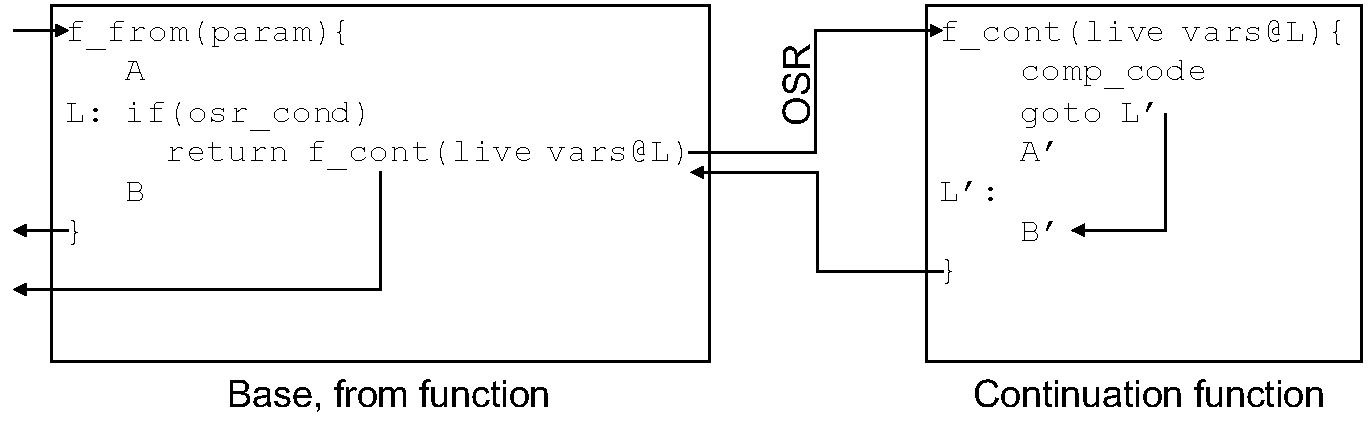
\includegraphics[scale=0.5]{Figures/OSRKitResolvedScenario}
\decoRule
\caption[Resolved OSR Scenario]{Resolved OSR scenario, from\cite{OSRKit}.}
\label{ResolvedOSRFig}
\end{figure}

Figure REF corresponds to the signature of the OSR Kit function that enables to insert resolved OSR.\\

\begin{minipage}{\linewidth}
\includecode{Code/ResolvedOSR.c}
\end{minipage}

The resolved OSR scenario does not require to inverse on the fly the transformations performed on the function and can therefore easily be used to implement the deoptimization case.
In order to obtain the optimized version of a function, one has to perform transformations on a base function.
This base function can therefore be used as the continuation function in the case of an OSR exit.
In RJIT, we rely on the resolved OSR to provide deoptimization of functions where call sites were inlined.
While generating the optimized version by speculatively inlining calls, the RJIT compiler introduces the OSR exit instrumentation with the base function as continuation function.
When several call sites are inlined, each of them is instrumented with an OSR exit that points to its own continuation function, which is a copy of the base function with the proper OSR instrumentation (see Section \ref{thecontinuationfunction}).\\



\section{The OSR Instrumentation}
\subsection{OSR Points \& Conditions}
%No distinction
%Both are done in the same way i.e., insert a condition.
%Do the condition testing, do the jump to a special block.
%Requirements for the point to be inserted !

In the OSR Kit library\cite{OSRKit}, there is no distinction at the implementation level between OSR exits and entries.
The general mechanism used is the OSR point.
An OSR point corresponds to a labelled LLVM basic-block that contains the call to the continuation function and the return instruction to propagate the result of the call.
OSR points are protected by an OSR condition. 
The OSR Kit library allows an OSR condition to be any vector of LLVM instructions. 
The last instruction is automatically used by the framework as condition for an LLVM branch instruction. 
If the condition succeeds, the OSR transition is fired.
Otherwise, the execution continues in the function.\\

Figures REF and REF provide an example of OSR instrumentation.
In Figure REF, we have the R declaration of two functions, $f$ and $g$, and the simplified LLVM IR generated for $g$ in RJIT.
Figure REF presents the instrumented version of $g$, in which an OSR point has been inserted.
Lines 5 and 6 correspond to the OSR condition.
In this example, the OSR is fired if line 1 does not yield the same function for $f$ as the one that was used by the RJIT compiler when it generated the instrumented function.
If the OSR is fired, the execution jumps to the \textit{OSR\char`_fire} basic block and calls the continuation function, namely \textit{OSRCont}.
The OSR point \textit{OSR\char`_fire} calls the continuation and propagates its return value line 15.
The \textit{OSR\char`_split} block corresponds to the regular continuation of the function $f$ when the OSR is not fired.\\

\begin{minipage}{\linewidth}
\includecode[asm]{Code/original.llvm}
\end{minipage}

\begin{minipage}{\linewidth}
\includecode[asm]{Code/fromInstrumented.llvm}
\end{minipage}

%TODO Requirements for a point.
REQUIREMENTS FOR OSR POINT\\

\subsection{The StateMap}

The OSR Kit library and our extensions heavily rely on a special object, called a \textit{StateMap}, to keep a mapping between the from function and the continuation function.
The StateMap enables to register unidirectional and bidirectional mappings between LLVM instructions and function arguments.
The default constructor for a StateMap relies on the LLVM ValueToValueMapTy\cite{VMap}(VMap) to automatically extract the mappings.
A VMap can be filled with such mappings when the LLVM cloning functions are used, i.e., the OSR Kit encourages you to generate the continuation function by cloning either the base or the from function such that a VMap is already available when the framework needs to introduce the instrumentation.
The StateMap also provides an API to register and unregister mappings by directly providing the two instructions.\\

%Transitive mappings
%Enables to skip versions!
In order to facilitate the use of StateMaps in the deoptimization case, we extended the object with transitive mappings.
Suppose two StateMaps, $S_1$ and $S_2$, such that $S_1$ is a mapping between $A$ and $B$, and $S_2$ a mapping between $A$ and $C$.
Our transitive constructor will be able to generate a new StateMap, $S_3$, that maps $B$ and $C$.
Consider a chained generation of versions, i.e., a succession of versions where each one of them is the result of some transformation applied on the previous version.
$$A \rightarrow B \rightarrow C \rightarrow D \rightarrow E \rightarrow F \rightarrow ...$$

The transitive StateMap constructor enables to automatically generate a transitive map between each versions in the chain.
The StateMap might not be complete, but it ensures that every instruction that is present in the base version $A$ and both versions that we want to map, e.g., $C$ and $F$, will be present in the StateMap.
WHY IT IS USEFUL !!!

\subsection{The continuation function}\label{thecontinuationfunction}
%The continuation function same in principle if we come from open or resolved. 
%Replaces the entry point of the function with a special OSR_ENtry block.
%CODE example
%block responsible for compensation code and jumping to the correct instruction, which is instrumented by the framework to be the head of a basic block. Everything before is deadcode, eliminated by LLVM automatically if optimizations are enabled.

%Live values are passed as arguments so no need to do any loading. Speed up the whole thing: quote from paper.

%In optimization -> optimize long running functions that's okay. Frequently called functions, a bit less. WHY
%In deoptimization, that is perfect if we do not expect to deoptimize frequently. 
%Got rid of that in RJIT by allowing the comp code to reset the closure corresponding to the function to actually contain the full deoptimzed method. TADA This is in the handler (see section bla). 

Both deoptimization and optimization rely on the same kind of continuation functions, and on the same instrumentation tools.
A continuation function, in OSR Kit, has a special function signature that takes as inputs all the variables that were live at the instruction at which the OSR transition was fired.
Its return type is the same as the from and the base (unmodified and un-instrumented) functions.
The OSR Kit instrumentation inserts a special basic block, called \textit{OSR ENTRY}, at the beginning of the continuation function.
The OSR ENTRY is responsible for executing a compensation code and jumping to the correct block inside the continuation function.
The compensation code is specified by the library user as a vector of instructions, when the OSR is inserted in the code.
The continuation instruction, i.e., the instruction to which the OSR ENTRY jumps to is assured by the OSR Kit library to be the first instruction in the destination block.
Everything between the OSR ENTRY and the continuation block becomes considered dead code.
The dead instructions are automatically eliminated by the LLVM transformation passes.
In any case, their only impact is on the space used up by the program, their presence does not increase the execution time of the continuation function.
It might, however, impact on later optimizations performed on the code.\\

CODE EXAMPLE.\\

Passing live values as arguments to the continuation function is more efficient than loading them from a buffer.
According to \cite{fink2003design}, generating a dedicated function to resume the execution to continue the execution, as opposed to instrument a general function to serve as continuation as well as a regular function, is expected to lead to better results.
In other words, it is supposed to be better to keep the base function to serve regular calls, and trigger OSR transitions whenever we need them, during the execution of the function.\\

In the case of long running functions, generating this type of OSR continuation function to transfer the execution to a more optimized version of the code makes sense.
The OSR entry is usually fired at some special control flow node, such as a function prologue or a loop header.
Therefore, the code expected to be repeatedly executed is not dead inside the continuation function.
On the other hand, the code leading to that portion, i.e., the code that needs to be executed only once or a few times, is dead code and does not matter.
It can therefore be removed without regret.
On the other hand, if the function is not a long running one, going through the cost of compiling the continuation function might overcome the benefits of the optimization. 
Nevertheless, if that is the case, a JIT compilation of the function should be used instead of the OSR mechanism.
If the optimization is based on an assumption that might fail, one can always JIT compile it with optimizations, and instrument it with OSR exits.\\

In the case of deoptimization, performance is a soft issue.
OSR exits are responsible for preserving correctness in the program. 
If an OSR exit is fired, the continuation function will be called.
Subsequent calls are still served by the optimized version of the function and might need to OSR exit too.
This can lead to a serious loss of performances.
For example, in the case of speculative call site inlining, an OSR exit is taken when the inlined function is redefined.
In subsequent calls, the same OSR exits will have to be taken.
With the OSR exit, the execution goes through an extra function call and return than in the unoptimized version.\\

In RJIT, when we know that an optimized version is no longer valid and will not be valid for subsequent calls either, we use the compensation code at the beginning of the continuation function to replace the optimized function in the environment with its unoptimized version.
The unoptimized version is a clone of the continuation function without the OSR instrumentation and with the same signature as the base function.
This mechanism is detailed in REF.
If we take the inlining example above, replacing the function with one that does not wrongly inline the call site is supposed to lead to better performances.\\


\section{Using OSR Kit to deoptimize}\label{osrForUs}
MIGHT MOVE THAT SOMEWHERE ELSE\\
\subsection{A case that does not fit perfectly}
PRESENT WHAT WE NEED TO CHANGE IN OSR KIT AND THE CHALLENGES.\\
%Cannot apply opposite of transformation so need to keep the base version somewhere. 
%Exit must be known in advance.
%Need to generate a lot of IR for a single function. 
%The OSR kit library works with a special continuation that cannot be used for regular calls, so need to be able to get this representation at some point for deopt and replace it.

%RJIT and the constants, instrumentations and other stuff on the side that makes it more difficult than just copying around the IR.
%Requires to clone a lot so increase the time spent in the compiler.
%One trick is to keep track of everything and reuse it as much as possible.

%Closures and what that implies. 
%Replacing the function. 

%As a conclusion, not exactly what we need here
Using OSR Kit 
 
\subsection{Where to exit?}
%What is possible and what is not
%Well can only exit to the previous version by default. BY DESIGN. 
%RJIT and transitive allow to make that more flexible, e.g., imagine there inlining
%Requires remapping of live values too.

\section{Extension in OSR RJIT}\label{extendingOSR}
%In this section details novel implementations, some of which we're referenced above.
%Added on top of the osr kit library, enables to better fit our use cases and also to enable to 
%switch from one design to another, experiment with different solutions etc. 

\subsection{The OSR Handler and function versions.}
%Takes care of the cloning and versioning 
%Provides simplified API to insert OSR points.
%Keeps track of statemaps.  
%Provides methods to update the statemap as we go, simple remove entries and add entries for now. 
%Future: would be great to have it wrap around the LLVM function and do all of that automatically, but that is a huge amount of work that we do not provide yet. 

\subsection{Fusing versions?}
%TRANSITIVE STATEMAPS
%Why do we want that ?
%it is a first step toward one continuation function, i.e., we can have the buffer implementation more easily 
%invalidate several assumptions at the same time -> e.g. inlining at the same level + reduces the number of versions that we keep in memory. 
    %What about the function signature? => take both sets and get union of them in the function signature, patch them will null values if they are not needed during the call. 
    %Implementation status .... wolololo


\subsection{Unguarded OSR points?}
%Keep track of stackmaps and patchpoints -> can enable this 

 
% Chapter 5

\chapter{Case Study: An R Inliner} % Main chapter title

\label{Chapter5} % For referencing the chapter elsewhere, use \ref{Chapter2} 

%----------------------------------------------------------------------------------------

% Define some commands to keep the formatting separated from the content 
\newcommand{\keyword}[1]{\textbf{#1}}
\newcommand{\tabhead}[1]{\textbf{#1}}
\newcommand{\code}[1]{\texttt{#1}}
\newcommand{\file}[1]{\texttt{\bfseries#1}}
\newcommand{\option}[1]{\texttt{\itshape#1}}

%----------------------------------------------------------------------------------------

\section{The RJIT project}
MOVE MEE TO RELATED WORK !!\\
\section{OSR in RJIT: requirements}
RENAME
REPLACE BY THE JITTED FUNCTION IF IT WAS NOT JITTED.
\section{Implementation}
\subsection{The Function Call in RJIT}
\subsection{Challenges}
\section{OSR Conditions}
 

%----------------------------------------------------------------------------------------
%	THESIS CONTENT - APPENDICES
%----------------------------------------------------------------------------------------

\appendix % Cue to tell LaTeX that the following "chapters" are Appendices

% Include the appendices of the thesis as separate files from the Appendices folder
% Uncomment the lines as you write the Appendices

% Appendix A

\chapter{Appendix Title Here} % Main appendix title

\label{AppendixA} % For referencing this appendix elsewhere, use \ref{AppendixA}

Write your Appendix content here.
%\input{Appendices/AppendixB}
%\input{Appendices/AppendixC}

%----------------------------------------------------------------------------------------
%	BIBLIOGRAPHY
%----------------------------------------------------------------------------------------

\printbibliography[heading=bibintoc]

%----------------------------------------------------------------------------------------

\end{document}